%% =====================================================================
%%  Elsevier version (target: Electric Power Systems Research,
%%  subscription route = NO author fee).  Class: elsarticle (preprint).
%%  Build:  latexmk -pdf main.tex      (bibtex style: elsarticle-num)
%% =====================================================================
\documentclass[preprint,12pt]{elsarticle}
\usepackage{amsmath,amssymb,amsfonts}
\usepackage{graphicx}
\usepackage{textcomp}
\usepackage{booktabs}
\usepackage{array}
\usepackage{multirow}
\usepackage{adjustbox}
\usepackage{xcolor}
\usepackage{url}
\usepackage{tikz}
\usetikzlibrary{arrows.meta,calc,positioning,shapes.geometric}

%% red marker for items the authors must fill in (delete before submission)
\newcommand{\todo}[1]{\textcolor{red}{[#1]}}
\newcommand{\kHz}{\,\text{kHz}}
\newcommand{\mA}{\,\text{mA}}
\newcommand{\Vdc}{V_{\mathrm{dc}}}
\newcommand{\Cpv}{C_{\mathrm{PV}}}
\newcommand{\Leq}{L_{\mathrm{eq}}}
\newcommand{\fsw}{f_{\mathrm{sw}}}
\newcommand{\fres}{f_{\mathrm{res}}}
\newcommand{\vCM}{v_{\mathrm{CM}}}
\newcommand{\vDM}{v_{\mathrm{DM}}}
\newcommand{\iCM}{i_{\mathrm{CM}}}
\hyphenation{trans-former-less}
\setlength{\emergencystretch}{4em}
\hfuzz=4pt
\usepackage{lineno}          % line numbers help reviewers (Elsevier recommends)
\newcommand{\IEEEPARstart}[2]{#1#2}   % sections use IEEE drop-cap macro; plain text here
\modulolinenumbers[5]
\journal{Electric Power Systems Research}

\begin{document}
\begin{frontmatter}

\title{Switching-frequency-dependent leakage current in H4 and HERIC transformerless PV inverters: a common-mode resonance perspective}

\author[kuet]{Razowan Kabir\corref{cor1}}
\ead{rkrazowan@gmail.com}
\author[kuet]{Mridha Raju}
\author[gstu]{Mursida Khatun}
\author[gstu]{Pantho Mondal}
\author[gstu]{Tanzim Khan}
\author[gstu]{Rabiul Islam}
\author[gstu]{A.T.M. Saiful Islam}

\cortext[cor1]{Corresponding author. ORCID: 0009-0008-6274-8117}

\affiliation[kuet]{organization={Department of Electrical and Electronic Engineering, Khulna University of Engineering and Technology},
            city={Khulna},
            country={Bangladesh}}
\affiliation[gstu]{organization={Department of Electrical and Electronic Engineering, Gopalganj Science and Technology University},
            city={Gopalganj},
            country={Bangladesh}}

\begin{abstract}
Transformerless single-phase inverters raise efficiency in grid-connected photovoltaic systems, but the missing galvanic isolation lets the switching common-mode voltage drive a leakage current through the parasitic capacitance between the photovoltaic array and ground. Safety standards require this current to stay below 300 mA. Most topology comparisons use a single switching frequency. This paper instead studies how the switching frequency interacts with the common-mode resonance formed by the output-filter inductance and the parasitic capacitance. Simulation models of the H4 inverter and the highly efficient and reliable inverter concept (HERIC), each with unipolar and bipolar sinusoidal pulse-width modulation, an inductive filter and a 150 nF parasitic capacitance, are swept from 1 kHz to 40 kHz while leakage current, efficiency and low-order harmonic distortion are recorded. In all four cases the leakage current peaks sharply, reaching about 0.75 A, 0.5 A and 4 A for H4 unipolar, H4 bipolar and HERIC unipolar, at frequencies that, for the dominant peaks, agree within about 5\% with the analytically predicted resonance, its sub-multiples or, in one case, twice its value. Elsewhere the leakage falls to 3.5--40~mA. With identical circuit parameters, bipolar HERIC leaks about eleven times less than unipolar HERIC, but its low-order distortion of about 9.1\% is high. The results are simulation-based and the H4 and HERIC parameter sets differ, so they support a switching-frequency selection rule (avoid the resonance, its sub-multiples and twice its value; prefer frequencies above 2.4 times the resonance) rather than a topology ranking.
\end{abstract}

\begin{highlights}
\item Leakage of H4 and HERIC inverters is swept over 1-40 kHz switching frequency
\item Leakage peaks match the resonance of filter inductance and PV capacitance
\item Effective common-mode source v\_CM - v\_o/2 explains the few-mA leakage floor
\item Simple rule: keep switching frequency away from the resonance and its multiples
\item Bipolar HERIC leaks 11 times less than unipolar HERIC but has 9\% low-order THD
\end{highlights}

\begin{keyword}
Common-mode voltage \sep H4 inverter \sep HERIC inverter \sep Leakage current \sep Parasitic capacitance \sep Photovoltaic systems \sep Switching frequency \sep Transformerless inverter
\end{keyword}

\end{frontmatter}

\linenumbers

%% Section 1: Introduction
\section{Introduction}
\label{sec:intro}
\IEEEPARstart{G}{rid-connected} photovoltaic (PV) generation is expanding rapidly, and the single-phase inverter is the component that largely determines conversion efficiency, cost and power quality at residential and commercial scale \cite{Kjaer2005}. Line-frequency or high-frequency transformers provide galvanic isolation between the PV array and the grid, but they add weight, cost and loss. Removing the transformer improves efficiency and power density \cite{Gonzalez2007,Araujo2010}, and transformerless inverters are therefore widely used in the low-power range.

The price of removing isolation is a conductive path between the PV array and the grid ground. The PV modules have a parasitic capacitance $\Cpv$ to the grounded frame and mounting structure, and this capacitance is in series with the inverter output filter and the grid impedance. Any time-varying CMV generated by the inverter drives a leakage current through $\Cpv$ \cite{Gubia2007,Lopez2007}. Such a current causes electromagnetic interference, additional loss, grid-current distortion and, above all, a shock hazard. Safety standards require disconnection when the continuous residual current exceeds 300~mA, and when it changes suddenly by specified steps within specified times \cite{VDE0126,IEC62109}.

The classical remedy is topological: H5, H6 and HERIC-type inverters decouple the PV array from the grid during the freewheeling intervals so that the CMV remains (ideally) constant \cite{Victor2008,Schmidt2003,Zhang2014,Kerekes2011}. In practice, however, the achieved leakage current depends on non-idealities and on the operating point. The switching frequency is of particular interest: it sets the filter size and the switching loss, but it also determines where the harmonics of the CMV fall relative to the CM resonance of the $L$--$\Cpv$ loop. This interaction is usually discussed qualitatively, and switching frequency is commonly chosen on the basis of efficiency and filter size alone.

\subsection{Contributions}
This paper makes the following contributions.
\begin{enumerate}
  \item A frequency-resolved simulation study (1--40~kHz) of the leakage current, efficiency and low-order THD of the H4 inverter with unipolar and bipolar sinusoidal PWM (SPWM) and of the HERIC inverter with unipolar and bipolar SPWM, using an L filter and a 150~nF parasitic capacitance.
  \item A CM-resonance interpretation of the results: in all four cases the leakage peaks occur where $\fsw$ coincides with a low-order sub-multiple of $\fres$ (or, in one case, with $2\fres$), where $\fres=1/(2\pi\sqrt{\Leq\Cpv})$ evaluated from the circuit parameters, and the leakage floor of the HERIC bipolar case is consistent with the line-frequency term $v_o/2$ of the effective CM source acting on $\Cpv$.
  \item A practical switching-frequency selection rule, together with a comparison of the operating windows that satisfy the 300~mA limit, and an explicit account of the limitations of the study (simulation only, non-uniform parameters between H4 and HERIC cases, band-limited THD).
\end{enumerate}

\subsection{Organization}
Section~\ref{sec:related} reviews related work and positions the study. Section~\ref{sec:cm} derives the CM model and the resonance condition. Section~\ref{sec:topologies} describes the topologies and modulation schemes. Section~\ref{sec:method} documents the simulation set-up and the metrics. Section~\ref{sec:results} presents the results, Section~\ref{sec:discussion} discusses the results, Section~\ref{sec:design} gives the sensitivity analysis and design guidelines, Section~\ref{sec:limits} states the limitations, and Section~\ref{sec:conclusion} concludes.

%% Section 2: Related work and positioning
\section{Related Work and Positioning}
\label{sec:related}

\subsection{Topologies for leakage-current suppression}
Early transformerless designs were based on the full-bridge (H4) inverter and its modulation variants \cite{Kjaer2005,Gonzalez2007}. With bipolar SPWM, the H4 CMV is ideally constant but the output is two-level, which increases the ripple and the filter requirement; with unipolar SPWM the output is three-level and more efficient, but the CMV switches at the carrier frequency \cite{Gonzalez2007,Gubia2007}. The H5 inverter adds a switch on the DC side so that the AC side is disconnected from the PV array during freewheeling \cite{Victor2008}; the HERIC inverter achieves the same decoupling with two switches on the AC side \cite{Schmidt2003}. The H6 family adds a second DC-side switch or a clamping network \cite{Zhang2014,Yu2011,Islam2015}. Mid-point-clamped bridges \cite{Kerekes2011}, common-ground structures \cite{Salem2021}, multilevel inverters \cite{Gonzalez2008} and further derivations \cite{Xiao2011} extend the family. Comprehensive topology reviews and derivation methodologies are given in \cite{Li2015,Khan2020,Kibria2023,Kolodziejski2023}.

\subsection{Modelling of leakage currents}
Equivalent CM circuits that include the parasitic capacitance, the filter inductances and the grid or ground impedance explain the main features of the leakage current \cite{Gubia2007,Lopez2007,Lopez2010}. More detailed parasitic-capacitor models improve the prediction of the leakage current \cite{Chen2016}, and the CM behavior of DC-decoupled and AC-decoupled topologies has been compared in \cite{Sundar2016}. A common conclusion is that leakage is governed by the magnitude and the spectral content of the total CMV and by the resonant impedance of the loop; the form of the CM transfer function used in this paper follows that of \cite{Gubia2007} and \cite{Shrestha2025}, with the source term adapted to the grounded-load circuit simulated here.

\subsection{Comparative studies and the gap addressed here}
Table~\ref{tab:related} summarizes recent comparative studies that are closest to the present work. Reference~\cite{Khan2020} compares major topologies analytically and by PLECS simulation, with cost, size, efficiency and thermal analysis; \cite{Kibria2023} simulates eighteen topologies with common parameters and reports the loss distribution; \cite{Kolodziejski2023} compares H4, H5, H6 and HERIC implemented with the same IGBTs in PSPICE; and \cite{Shrestha2025} compares H4, H5 and HERIC in MATLAB/\-Simulink and concludes that H5 offers the best balance between leakage current, THD and efficiency. These studies are primarily topology-centric. To the best of the authors' knowledge, and on the basis of the studies reviewed here, the explicit dependence of the leakage current on the \emph{switching frequency}, and the relation of leakage peaks to the CM resonance of the filter and the parasitic capacitance, receive less systematic attention. This is the gap that the present paper addresses, for the H4 and HERIC inverters under unipolar and bipolar SPWM. A systematic search for frequency-sweep studies should accompany the final submission (see the notes accompanying this manuscript).

\begin{table*}[!t]
\renewcommand{\arraystretch}{1.2}
\caption{Closest comparative studies and the position of this work}
\label{tab:related}
\centering
\footnotesize
\begin{adjustbox}{max width=\textwidth}
\begin{tabular}{p{1.4cm}p{3.0cm}p{2.6cm}p{6.2cm}}
\toprule
Ref. & Topologies & Tool & Main conclusion / focus \\
\midrule
\cite{Li2015} & Derivation and review of leakage-suppressing topologies & Review & Systematic derivation methodology \\
\cite{Khan2020} & Major single-phase transformerless topologies & Analysis, PLECS & CM behavior, cost, size, efficiency, thermal analysis, roadmap \\
\cite{Kibria2023} & Eighteen topologies & MATLAB/\-Simulink & Common parameters, IGBT switches, loss distribution per switch \\
\cite{Kolodziejski2023} & H4, H5, H6, HERIC & PSPICE & Same components and parameters; efficiency and leakage \\
\cite{Shrestha2025} & H4, H5, HERIC & MATLAB/\-Simulink & H5 gives best balance of leakage, THD and efficiency \\
This work & H4 and HERIC, unipolar and bipolar SPWM & MATLAB/\-Simulink & Frequency sweep 1--40~kHz; CM-resonance interpretation; frequency-selection rule \\
\bottomrule
\end{tabular}
\end{adjustbox}
\end{table*}

\subsection{Filters, modulation and standards}
The output filter shapes both the grid-current quality and the CM path. LCL filters give higher harmonic attenuation than L filters at the same inductance and are the usual choice for grid-connected inverters, and systematic design procedures exist \cite{Reznik2014}; in a transformerless inverter, however, the shunt capacitance of an LC or LCL filter, when referred to the grounded neutral, adds a high-frequency CM path, which is why the L filter is attractive for leakage studies. Unipolar modulation reduces the ripple seen by the filter relative to bipolar modulation \cite{Gonzalez2007,Salem2021}, which is the reason for its higher efficiency, and the topologies that preserve this advantage while keeping $\vCM$ constant are the main subject of the topology literature above.

The applicable standards combine safety and power-quality requirements. The leakage current is regulated by VDE~V~0126-1-1 and IEC~62109-2 \cite{VDE0126,IEC62109}; the comparative review \cite{Khan2020} lists IEEE~1547.1, VDE~0126-1-1, EN~50106, IEC~61727 and AS/NZS~5033 as the standards that transformerless inverters must comply with in different regions. The harmonic distortion at the point of connection is governed by IEEE~1547 and IEEE~519 \cite{IEEE1547,IEEE519}. The present study addresses the first group directly and the second only through a low-order THD.

\subsection{Problem statement}
Let a transformerless inverter with topology $\mathcal{T}$ and modulation $\mathcal{M}$ feed a load through an L filter of inductance $L$ in the presence of a parasitic capacitance $\Cpv$. For a given operating point, let $I_{\mathrm{leak}}(\fsw)$, $\eta(\fsw)$ and $\mathrm{THD}(\fsw)$ denote the RMS leakage current, the efficiency and the low-order THD. The question addressed is the following: for which switching frequencies does $I_{\mathrm{leak}}(\fsw)$ fall below the limit of 300~mA with margin, how does this set depend on $(\mathcal{T},\mathcal{M})$, and can its complement (the frequencies to be avoided) be predicted from $L$ and $\Cpv$ alone? The scope is deliberately restricted to the inverter stage and its CM path; control loops, MPPT and grid-impedance effects are excluded.

%% Section 3: Common-mode model and resonance condition
\section{Common-Mode Model and Resonance Condition}
\label{sec:cm}
Fig.~\ref{fig:schematic} shows the generic power stage used in this study: a DC source with a DC-link capacitor, a full bridge, an optional HERIC AC bypass, an L filter, a resistive load across the filter output whose lower terminal is earthed, and the parasitic capacitance $\Cpv$ between the negative DC rail and ground.

\begin{figure}[!t]
\centering
\resizebox{\columnwidth}{!}{%
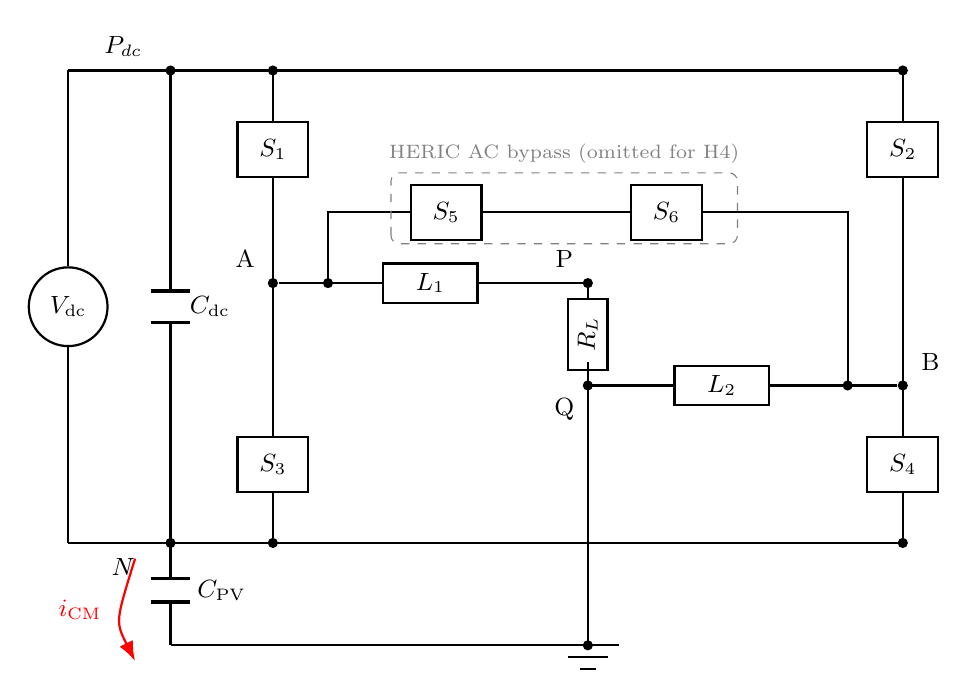
\begin{tikzpicture}[x=1cm,y=1cm,font=\small,
  sw/.style={draw,thick,minimum width=9mm,minimum height=7mm,fill=white},
  bx/.style={draw,thick,minimum width=12mm,minimum height=5mm,fill=white},
  jn/.style={circle,fill,inner sep=1.3pt}]
% DC rails
\draw[thick] (-2.6,5)--(8,5); \draw[thick] (-2.6,-1)--(8,-1);
\node[circle,draw,thick,minimum size=10mm] (V) at (-2.6,2) {$V_{\mathrm{dc}}$};
\draw[thick] (V.north)--(-2.6,5); \draw[thick] (V.south)--(-2.6,-1);
% DC-link capacitor
\draw[thick] (-1.3,5)--(-1.3,2.2); \draw[very thick] (-1.55,2.2)--(-1.05,2.2);
\draw[very thick] (-1.55,1.8)--(-1.05,1.8); \draw[thick] (-1.3,1.8)--(-1.3,-1);
\node[jn] at (-1.3,5) {}; \node[jn] at (-1.3,-1) {};
\node at (-0.8,2.0) {$C_{\mathrm{dc}}$};
% legs
\node[sw] at (0,4.0) {$S_1$}; \node[sw] at (0,0.0) {$S_3$};
\node[sw] at (8,4.0) {$S_2$}; \node[sw] at (8,0.0) {$S_4$};
\draw[thick] (0,5)--(0,4.35); \draw[thick] (0,3.65)--(0,0.35); \draw[thick] (0,-0.35)--(0,-1);
\draw[thick] (8,5)--(8,4.35); \draw[thick] (8,3.65)--(8,0.35); \draw[thick] (8,-0.35)--(8,-1);
\node[jn] at (0,5) {}; \node[jn] at (0,-1) {}; \node[jn] at (8,5) {}; \node[jn] at (8,-1) {};
% filter: A - L1 - P ; B - L2 - Q ; R_L between P and Q ; Q grounded
\node[jn] (A) at (0,2.3) {}; \node at (-0.35,2.6) {A};
\node[jn] (B) at (8,1.0) {}; \node at (8.35,1.3) {B};
\draw[thick] (A)--(1.4,2.3); \node[bx] at (2.0,2.3) {$L_1$}; \draw[thick] (2.6,2.3)--(4,2.3);
\node[jn] (P) at (4,2.3) {}; \node at (3.7,2.6) {P};
\draw[thick] (B)--(6.3,1.0); \node[bx] at (5.7,1.0) {$L_2$}; \draw[thick] (5.1,1.0)--(4,1.0);
\node[jn] (Q) at (4,1.0) {}; \node at (3.7,0.7) {Q};
\draw[thick] (4,2.3)--(4,2.0); \node[draw,thick,minimum width=5mm,minimum height=9mm,fill=white,font=\small] at (4,1.65) {\rotatebox{90}{$R_L$}};
\draw[thick] (4,1.3)--(4,1.0);
% HERIC bypass
\node[jn] at (0.7,2.3) {}; \node[jn] at (7.3,1.0) {};
\node[sw] (S5) at (2.2,3.2) {$S_5$}; \node[sw] (S6) at (5.0,3.2) {$S_6$};
\draw[thick] (0.7,2.3)--(0.7,3.2)--(S5.west); \draw[thick] (S5.east)--(S6.west);
\draw[thick] (S6.east)--(7.3,3.2)--(7.3,1.0);
\draw[dashed,rounded corners=3pt,gray] (1.5,2.8) rectangle (5.9,3.7);
\node[gray,font=\scriptsize] at (3.7,3.95) {HERIC AC bypass (omitted for H4)};
% parasitic capacitance, ground
\draw[thick] (4,1.0)--(4,-2.3);
\draw[thick] (-1.3,-1)--(-1.3,-1.45); \draw[very thick] (-1.55,-1.45)--(-1.05,-1.45);
\draw[very thick] (-1.55,-1.75)--(-1.05,-1.75); \draw[thick] (-1.3,-1.75)--(-1.3,-2.3);
\node at (-0.65,-1.6) {$C_{\mathrm{PV}}$};
\draw[thick] (-1.3,-2.3)--(4,-2.3); \node[jn] at (4,-2.3) {};
\draw[thick] (3.6,-2.3)--(4.4,-2.3); \draw[thick] (3.75,-2.45)--(4.25,-2.45); \draw[thick] (3.9,-2.6)--(4.1,-2.6);
\draw[-{Latex[length=2.5mm]},thick,red] (-1.75,-1.2) .. controls (-2.0,-2.0) .. (-1.75,-2.5);
\node[red] at (-2.45,-1.85) {$i_{\mathrm{CM}}$};
\node at (-1.9,5.3) {$P_{dc}$}; \node at (-1.9,-1.3) {$N$};
\end{tikzpicture}}
\caption{Power stage used in the study. The bridge ($S_1$--$S_4$, each with an anti-parallel diode) feeds two filter inductors $L_1$, $L_2$ and a resistive load $R_L$ connected between P and Q; node Q (the load's lower terminal) is grounded. The HERIC variant adds the AC bypass $S_5$, $S_6$ between nodes A and B. $\Cpv$ is the parasitic capacitance between the negative DC rail $N$ and ground; the leakage current $\iCM$ closes through $\Cpv$.}
\label{fig:schematic}
\end{figure}

\subsection{Pole voltages, CMV and differential-mode voltage}
Let $v_{AN}$ and $v_{BN}$ be the pole voltages of the two bridge legs with respect to the negative DC rail $N$. The CMV and the differential-mode voltage (DMV) are
\begin{equation}
\vCM=\frac{v_{AN}+v_{BN}}{2},\qquad \vDM=v_{AN}-v_{BN}.
\label{eq:cmdm}
\end{equation}
The DMV is the voltage that produces the load current; the CMV is the average of the two poles. With the load's lower terminal grounded (the role played by the grid neutral in a grid-connected system) and $L_1=L_2$, the voltage that actually drives the PV-to-ground loop is not $\vCM$ alone. Applying Kirchhoff's voltage law to the two filter branches (Appendix~\ref{app:cm}) gives the effective CM source
\begin{equation}
e(t)=\vCM(t)-\frac{v_o(t)}{2},
\label{eq:tcm}
\end{equation}
where $v_o$ is the voltage across the load. The second term is a line-frequency component of amplitude equal to half the output-voltage amplitude; it is present for every H-bridge variant, however ideal its $\vCM$. For unequal inductances, the general form $v_{tCM}=\vCM+\tfrac{\vDM}{2}\tfrac{L_2-L_1}{L_1+L_2}$ applies when the ground reference is at the midpoint of the DM path \cite{Gubia2007,Shrestha2025}.

\subsection{Equivalent CM circuit and resonance}
The CM current returns through the two filter branches in parallel (via $L_2$ directly and via $R_L$ and $L_1$) and closes through $\Cpv$. The equivalent CM circuit is therefore the series connection of $\Leq=L_1L_2/(L_1+L_2)=L/2$ and $\Cpv$ driven by $e(t)$ (Fig.~\ref{fig:cmcircuit}; the load resistance is already accounted for by the term $v_o/2$ in \eqref{eq:tcm}, and resistive loss in the loop is neglected). The CM current is then
\begin{align}
\iCM(s)&=\frac{e(s)}{s\Leq+1/(s\Cpv)},\label{eq:icm}\\
\fres&=\frac{1}{2\pi\sqrt{\Leq\Cpv}}.\label{eq:fres}
\end{align}
Two regimes follow. If $\vCM$ is constant and $v_o$ is a pure sinusoid, $e(t)$ contains only a 50-Hz component, and the leakage is the small displacement current of that component, which is capacitive well below $\fres$:
\begin{equation}
I_{\mathrm{floor}}\approx\frac{\omega_g\,\Cpv\,V_{o,pk}}{2\sqrt{2}},\qquad \omega_g=2\pi\cdot 50~\mathrm{rad/s},
\label{eq:floor}
\end{equation}
where $V_{o,pk}$ is the amplitude of the fundamental output voltage. If $\vCM$ contains components at the carrier frequency or its multiples, the corresponding leakage components are amplified by $1/|\omega\Leq-1/(\omega\Cpv)|$, which has a pole at $\fres$. In a switched converter, $\vCM$ contains components at $k\fsw$ whenever it is not perfectly constant, so leakage peaks are expected when $k\fsw\approx\fres$ for integer $k$ (with weight decreasing with $k$). A peak at $\fsw\approx2\fres$ is not predicted by this mechanism, because it would require sub-harmonic content at $\fsw/2$ in $e(t)$; one such peak appears in the H4 bipolar sweep (Section~\ref{sec:results}) and is treated as an empirical feature. Well above resonance the loop is inductive and the leakage decreases as $1/f$.

\begin{figure}[!t]
\centering
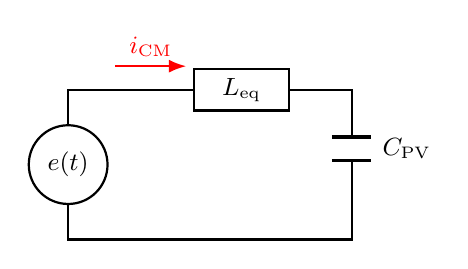
\begin{tikzpicture}[font=\small]
\node[circle,draw,thick,minimum size=10mm] (V) at (0,0) {$e(t)$};
\draw[thick] (V.north)--(0,0.95)--(1.6,0.95);
\node[draw,thick,minimum width=12mm,minimum height=5mm,fill=white] (L) at (2.2,0.95) {$\Leq$};
\draw[thick] (L.east)--(3.6,0.95)--(3.6,0.35);
\draw[very thick] (3.35,0.35)--(3.85,0.35); \draw[very thick] (3.35,0.05)--(3.85,0.05);
\draw[thick] (3.6,0.05)--(3.6,-0.95)--(0,-0.95)--(V.south);
\node at (4.3,0.2) {$\Cpv$};
\draw[-{Latex[length=2.2mm]},thick,red] (0.6,1.25)--(1.5,1.25);
\node[red] at (1.05,1.5) {$\iCM$};
\end{tikzpicture}
\caption{First-order CM equivalent circuit. $e(t)=\vCM-v_o/2$ is the effective CM source, $\Leq=L_1L_2/(L_1+L_2)$ is the parallel combination of the filter inductances and $\Cpv$ is the PV-to-ground parasitic capacitance.}
\label{fig:cmcircuit}
\end{figure}

\subsection{Safety limits}
The leakage current is limited by VDE~V~0126-1-1 and IEC~62109-2: for inverters up to 30~kVA the inverter must disconnect within 0.3~s if the continuous residual current exceeds 300~mA, and within 300~ms, 150~ms and 40~ms for sudden changes of 30~mA, 60~mA and 150~mA, respectively \cite{VDE0126,IEC62109}. In this paper the RMS leakage current is compared against the 300~mA continuous limit; the sudden-change limits require a time-domain evaluation with a control-and-protection model that is outside the scope of this study.

%% Section 4: Topologies and modulation
\section{Topologies and Modulation}
\label{sec:topologies}

\subsection{H4 inverter}
The H4 inverter comprises four switches $S_1$--$S_4$ with anti-parallel diodes (Fig.~\ref{fig:schematic} without $S_5$, $S_6$). The pairs $(S_1,S_4)$ and $(S_2,S_3)$ are the diagonal pairs that deliver positive and negative output voltage, respectively.

\emph{Bipolar SPWM:} a sinusoidal reference is compared with a triangular carrier; the diagonal pairs are switched complementarily at $\fsw$. The output alternates between $+\Vdc$ and $-\Vdc$ (two levels) and, ideally, $\vCM=\Vdc/2$ at all times.

\emph{Unipolar SPWM:} the legs are modulated with sinusoidal references of opposite sign. The output has three levels ($+\Vdc$, $0$, $-\Vdc$), which halves the effective ripple frequency seen by the filter and improves efficiency, but the freewheeling states connect both poles to the same rail so that $\vCM$ steps between $0$, $\Vdc/2$ and $\Vdc$ at the carrier frequency (Table~\ref{tab:cmv}).

\subsection{HERIC inverter}
The HERIC inverter adds two switches $S_5$, $S_6$ with diodes between the bridge output nodes A and B on the AC side \cite{Schmidt2003}. During the active intervals the bridge delivers $\pm\Vdc$ as in the H4 inverter; during the zero-voltage intervals all bridge switches are off and the filter current freewheels through the AC bypass ($S_5$ for one polarity, $S_6$ for the other), which disconnects the AC side from the PV array. Because the DC side then floats, the CMV remains, ideally, at $\Vdc/2$ in all four operating states, which is the origin of the low-leakage property \cite{Araujo2010,Sundar2016}. In real circuits the decoupling is imperfect owing to the parasitic capacitances of the switches and to dead time, so a residual CMV component remains.

\begin{table}[!t]
\renewcommand{\arraystretch}{1.2}
\caption{Ideal CMV behavior of the configurations studied}
\label{tab:cmv}
\centering
\footnotesize
\begin{adjustbox}{max width=\columnwidth}
\begin{tabular}{p{3.0cm}p{2.8cm}p{2.4cm}p{3.0cm}}
\toprule
Configuration & Output levels & Ideal $\vCM$ & Carrier-frequency content of $\vCM$ \\
\midrule
H4, bipolar SPWM & 2 ($\pm\Vdc$) & $\Vdc/2$ & None (ideal) \\
H4, unipolar SPWM & 3 ($\pm\Vdc$, 0) & $0$, $\Vdc/2$, $\Vdc$ & Yes \\
HERIC, unipolar SPWM & 3 ($\pm\Vdc$, 0) & $\Vdc/2$ & None (ideal) \\
HERIC, bipolar SPWM & 2 ($\pm\Vdc$) with bypass & $\Vdc/2$ & None (ideal) \\
\bottomrule
\end{tabular}
\end{adjustbox}
\end{table}

The ``HERIC bipolar'' configuration studied here applies bipolar SPWM to the bridge while the bypass switches are driven at line frequency; it is not the conventional HERIC modulation, which uses unipolar PWM, and it is included as a variant because it was found to give the lowest leakage in the simulations.

\subsection{Modulation and ripple considerations}
In SPWM the switching signals are generated by comparing a sinusoidal reference $v_r=m_a\sin(\omega t)$, $0<m_a\le1$, with a triangular carrier of frequency $\fsw$ and unit amplitude. For bipolar SPWM a single reference drives the diagonal pairs complementarily; for unipolar SPWM the references $+v_r$ and $-v_r$ drive the two legs separately, so that the bridge output has three levels and its spectrum is centered on $2\fsw$ rather than $\fsw$. For a single bridge leg the duty cycle is $D(\omega t)=m_a\sin(\omega t)$ and the inductor current ripple is
\begin{equation}
\Delta I_{pp}=\frac{D\,T_s\,(\Vdc-V_{o})}{L},\qquad V_o=\Vdc D,
\label{eq:ripple}
\end{equation}
whose maximum with respect to the duty cycle, at $D=1/2$, gives $\Delta I_{pp,\max}=\Vdc/(4\fsw L)$. This bound is useful in this study because the leakage-current sweep spans a ratio of 40 in $\fsw$: at the lowest frequencies the ripple, and hence the low-order THD, is large (Section~\ref{sec:results}). The design rules for LCL filters in \cite{Reznik2014} (total inductance limited to about 10\% of the base impedance, shunt capacitor absorbing about 5\% of the rated reactive power, and the resonance placed between $10f_g$ and $0.5\fsw$) are reproduced here only for context, since the L filter used in this study has no shunt branch.

\subsection{Choice of output filter}
An L filter was adopted. Shunt capacitors in LC and LCL filters reduce the harmonic content more effectively, and \cite{Reznik2014} provides the corresponding design rules (e.g., a resonance between ten times the grid frequency and half the switching frequency). However, a shunt capacitor referred to the grounded neutral adds a high-frequency CM path, and it complicates the CM model of Section~\ref{sec:cm}. The L filter keeps the CM impedance determined by $\Leq$ alone and thus isolates the effect of the switching frequency. The inductor ripple at the worst case follows the standard result $\Delta I_{pp,\max}=\Vdc/(4\fsw L)$, from which $L$ can be chosen for a given ripple limit at the lowest swept frequency. A comparison with LC and LCL filters is left for future work.

%% Section 5: Simulation methodology
\section{Simulation Methodology}
\label{sec:method}

\subsection{Models and parameters}
All models were built in MATLAB/Simulink with the Simscape Electrical (Powergui) continuous solver. Each model contains a DC source with series resistance $R_{dc}=0.049\;\Omega$ and a DC-link capacitor $C_{dc}=0.94$~F (as simulated), the bridge, the HERIC bypass where applicable, an L filter with $L_1=L_2=L$, a resistive load $R_L$ with its lower terminal grounded, and a parasitic capacitance $\Cpv=150$~nF between the negative DC rail and ground (Fig.~\ref{fig:model}). The value of $\Cpv$ lies within the 50--150~nF/kW range commonly quoted for crystalline modules. The leakage current is the current through $\Cpv$, measured with a current sensor and reported as an RMS value. The load is resistive and the model contains no grid source, current controller or phase-locked loop; the grounded load terminal plays the role of the grounded grid neutral, which is the reference that defines the CM loop. Table~\ref{tab:params} lists the parameters of the four cases.

\begin{table*}[!t]
\renewcommand{\arraystretch}{1.2}
\caption{Simulation parameters of the four cases ($\Cpv=150$~nF, $C_{dc}=0.94$~F, $R_{dc}=0.049\;\Omega$ in all cases)}
\label{tab:params}
\centering
\footnotesize
\resizebox{\textwidth}{!}{%
\begin{tabular}{lccccccccc}
\toprule
Case & $\Vdc$ (V) & $L_1=L_2$ & $R_L$ ($\Omega$) & $X_L/R_L$$^{c}$ & Est.\ $P_o$ (kW)$^{a}$ & Sweep (kHz) & $\Leq$ (mH) & $\fres$ (kHz) & Switch model$^{b}$ \\
\midrule
H4, unipolar   & 220 & 90~mH & 50    & 1.13 & 0.5 & 1--25 & 45 & 1.94 & MOSFET \\
H4, bipolar    & 460 & 10~mH & 10    & 0.63 & 7.4 & 1--40 & 5  & 5.81 & IGBT \\
HERIC, unipolar & 220 & 10~mH & 10.68 & 0.59 & 1.7 & 5--30 & 5  & 5.81 & IGBT \\
HERIC, bipolar  & 220 & 10~mH & 10.68 & 0.59 & 1.7 & 5--35 & 5  & 5.81 & IGBT \\
\bottomrule
\end{tabular}}\\[2pt]
\begin{minipage}{0.97\textwidth}\footnotesize
$^{c}$Series reactance of $L_1+L_2$ at 50~Hz relative to $R_L$. $^{a}$Estimated from the fundamental amplitude of the output voltage in the FFT results and $R_L$; \todo{confirm with the actual measured output power}. $^{b}$As listed in the simulation records; \todo{confirm device models and their on-state/switching parameters for each case}.
\end{minipage}
\end{table*}

\begin{figure}[!t]
\centering
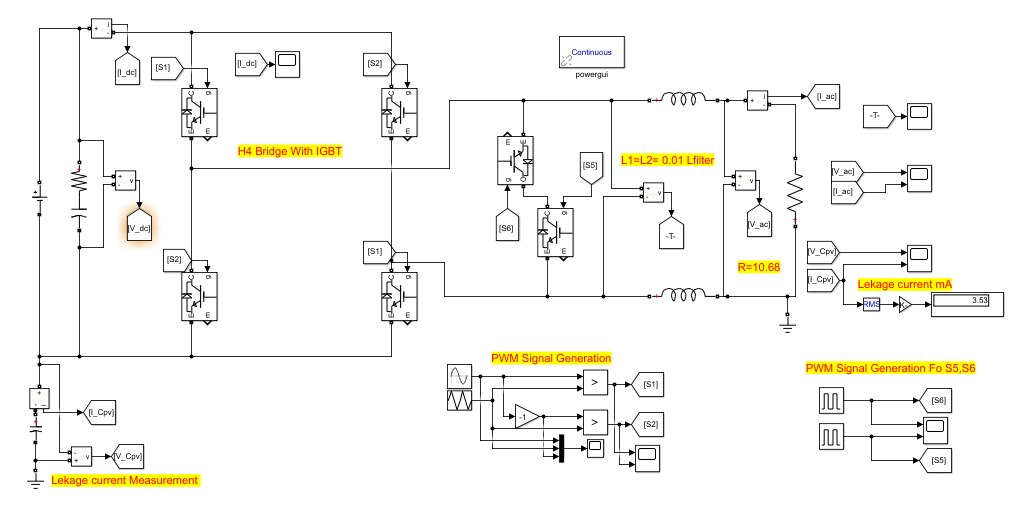
\includegraphics[width=\columnwidth]{figures/model_heric_bipolar.jpg}
\caption{Simulink model of the HERIC bipolar case. The H-bridge (IGBTs), the AC bypass ($S_5$, $S_6$), the L filter ($L_1=L_2=0.01$~H), the 10.68~$\Omega$ load with grounded lower terminal and the leakage-current measurement through $\Cpv$ are visible. The RMS leakage current is displayed in mA.}
\label{fig:model}
\end{figure}

The resonance frequencies in Table~\ref{tab:params} follow directly from~\eqref{eq:icm}: $\Leq=45$~mH gives $\fres=1.94$~kHz and $\Leq=5$~mH gives $\fres=5.81$~kHz.

\subsection{Metrics}
\emph{Leakage current:} RMS value of the current through $\Cpv$, compared with the 300~mA limit. \emph{Efficiency:} $\eta=P_o/P_{in}$ from the measured DC input and AC output powers; as the switch models include only their on-state and diode parameters, $\eta$ reflects conduction-type loss and does not constitute a complete switching-loss or thermal assessment. \emph{THD:} computed by the Powergui FFT tool on the load voltage (for a resistive load, voltage and current THD are identical), with the fundamental at 50~Hz. The tool was configured for harmonic orders up to the 40th (2~kHz); hence the reported THD is a \emph{low-order} THD that excludes the switching-frequency sidebands, which are attenuated by the filter and are addressed by the standards separately. Observation windows were 2--5 fundamental cycles after the start-up transient (stop time 0.05--0.08~s).

\subsection{Sweeps}
For each case the switching frequency was swept in steps of 0.5--1~kHz at low frequencies and in larger steps above 20~kHz, with the other parameters constant. The resulting resolution (0.5--1~kHz near the resonance) limits the accuracy with which the peak position can be located to about $\pm 0.5$~kHz.

\subsection{Study workflow and post-processing}
Fig.~\ref{fig:workflow} summarizes the procedure applied to each of the four cases. The analytical resonance $\fres$ was computed from \eqref{eq:fres} before the simulations were run, so that the comparison with the sweep results is a prediction and not a fit. For every switching frequency in the sweep, the model was run to the stop time of Table~\ref{tab:repro}, and three metrics were extracted from the last 2--5 fundamental cycles: the RMS value of the current through $\Cpv$, the efficiency from the DC input and AC output powers, and the low-order THD from the Powergui FFT tool. Leakage peaks were identified as local maxima of the leakage-versus-frequency curve in the sweep plots, and the deviation of a peak from the prediction was defined as the difference between the peak frequency and the nearest predicted frequency among $\fres$, $\fres/2$, $\fres/3$ and $2\fres$, relative to that predicted frequency (Table~\ref{tab:res}). The selection rule of Section~\ref{sec:design} was derived from these deviations and from the width of the observed peaks, and was not optimized against any additional data.

\begin{figure}[!t]
\centering
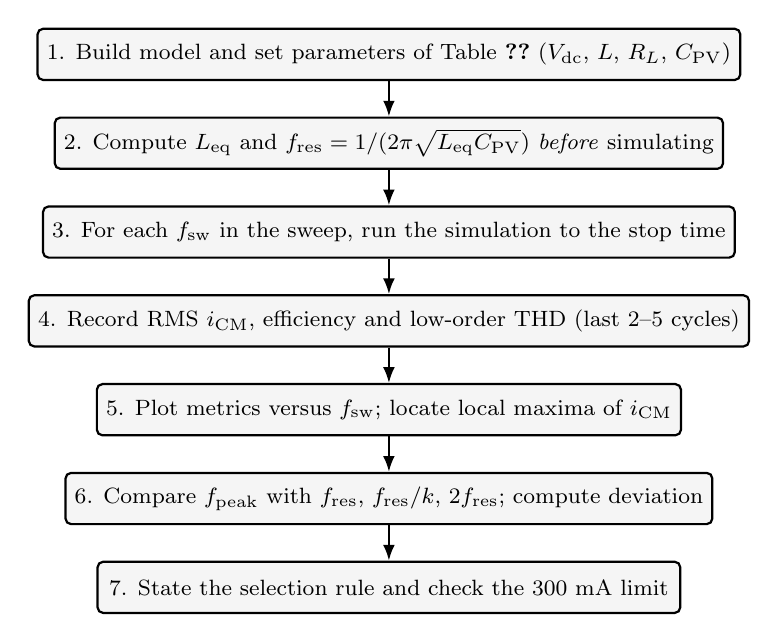
\begin{tikzpicture}[font=\footnotesize,node distance=4.5mm,
 blk/.style={draw,thick,rounded corners=2pt,minimum width=7.4cm,minimum height=6.5mm,align=center,fill=gray!8},
 arr/.style={-{Latex[length=2mm]},thick}]
\node[blk] (a) {1. Build model and set parameters of Table~\ref{tab:params} ($\Vdc$, $L$, $R_L$, $\Cpv$)};
\node[blk,below=of a] (b) {2. Compute $\Leq$ and $\fres=1/(2\pi\sqrt{\Leq\Cpv})$ \emph{before} simulating};
\node[blk,below=of b] (c) {3. For each $\fsw$ in the sweep, run the simulation to the stop time};
\node[blk,below=of c] (d) {4. Record RMS $\iCM$, efficiency and low-order THD (last 2--5 cycles)};
\node[blk,below=of d] (e) {5. Plot metrics versus $\fsw$; locate local maxima of $\iCM$};
\node[blk,below=of e] (f) {6. Compare $f_{\mathrm{peak}}$ with $\fres$, $\fres/k$, $2\fres$; compute deviation};
\node[blk,below=of f] (g) {7. State the selection rule and check the 300~mA limit};
\foreach \x/\y in {a/b,b/c,c/d,d/e,e/f,f/g} \draw[arr] (\x.south)--(\y.north);
\end{tikzpicture}
\caption{Study workflow applied to each of the four cases.}
\label{fig:workflow}
\end{figure}

%% Section 6: Results and discussion
\section{Results and Discussion}
\label{sec:results}

\subsection{H4 inverter with unipolar SPWM}
Fig.~\ref{fig:sweepH4U} shows the sweep from 1 to 25~kHz with $L=90$~mH. The leakage current has a sharp peak at 2~kHz, of the order of 0.75~A (the vertical axis of the plot is in amperes; \todo{relabel the axis of the figure as ``A'' or rescale to mA before submission}), accompanied by a dip in efficiency to about 97.0\% and a low-order THD of about 18\%. The peak lies within 3\% of the predicted resonance $\fres=1.94$~kHz. For $\fsw\geq3$~kHz the leakage decays rapidly; at 8.5~kHz it is 15.4~mA with an efficiency of 97.18\% and a THD of 0.16\% (Fig.~\ref{fig:fftH4B} shows a representative FFT for another case). The efficiency is essentially constant (97.2\%) for $\fsw>3$~kHz, which again indicates that switching loss is not modeled in this case. The leakage current falls below 300~mA everywhere except in the neighborhood of the resonance.

\begin{figure*}[!t]
\centering
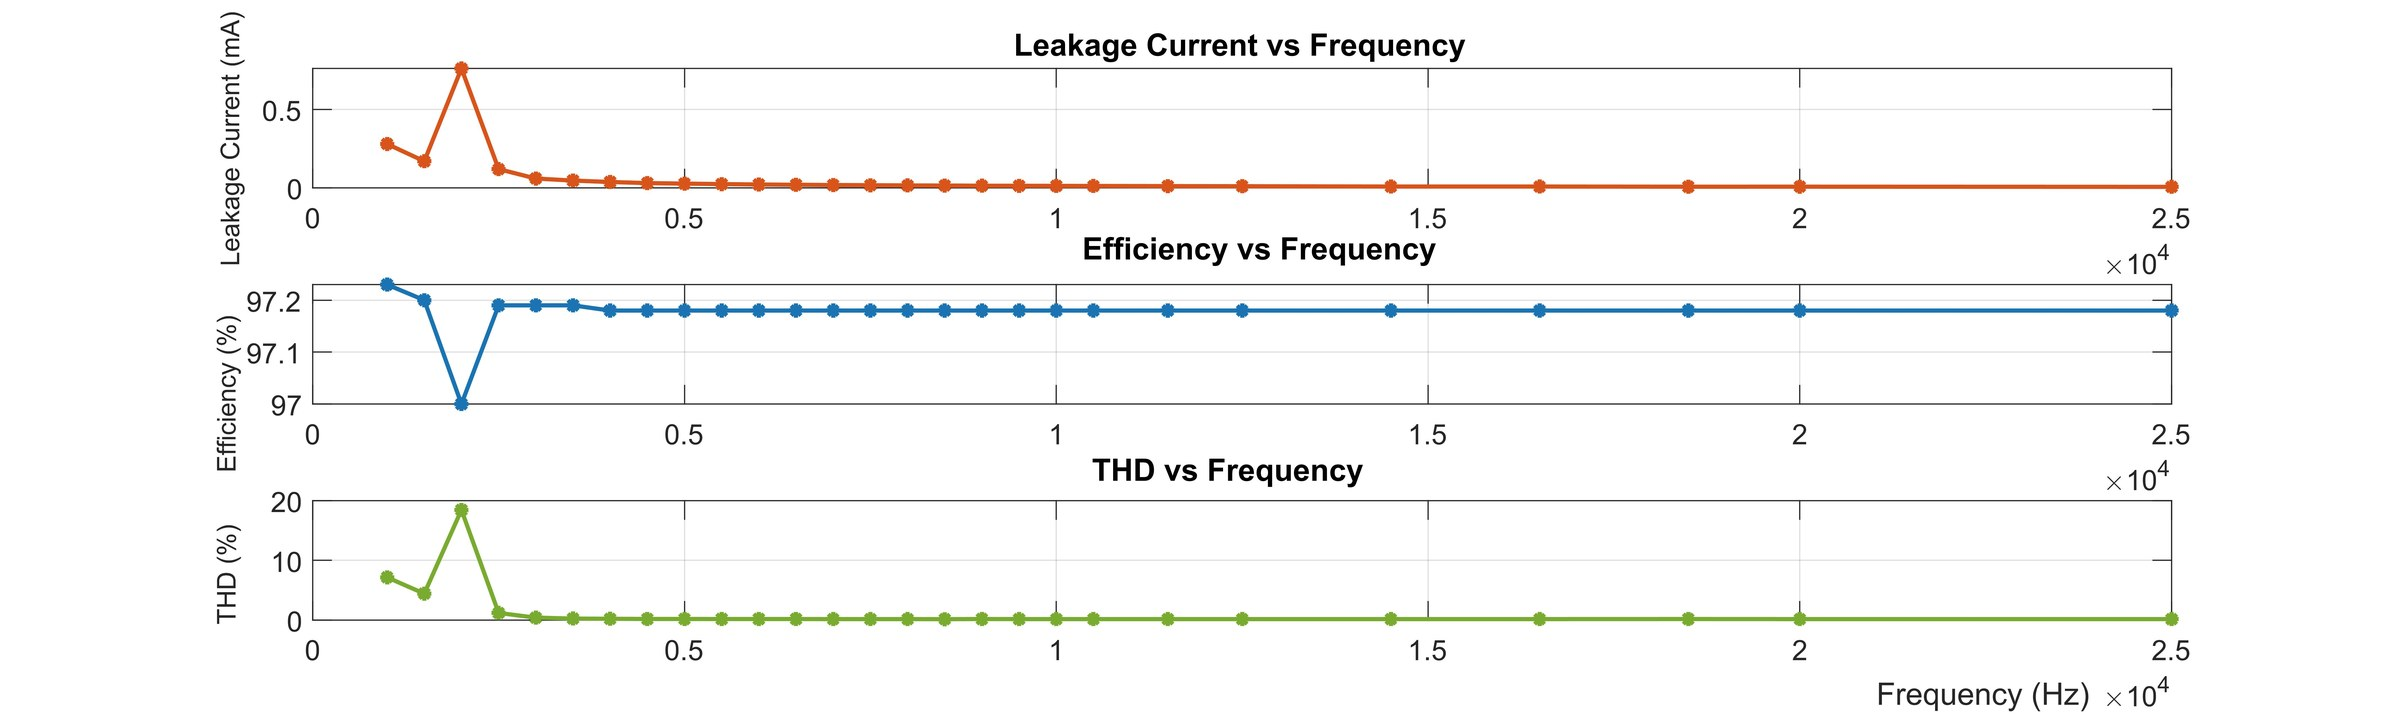
\includegraphics[width=0.85\textwidth]{figures/sweep_h4_unipolar.jpg}
\caption{H4 with unipolar SPWM: leakage current, efficiency and low-order THD versus switching frequency ($\Vdc=220$~V, $L_1=L_2=90$~mH, $R_L=50\;\Omega$, $\Cpv=150$~nF). \todo{The leakage axis is labelled mA in the source plot but its values correspond to amperes; correct before submission.}}
\label{fig:sweepH4U}
\end{figure*}

The CMV and leakage waveforms at the start of the simulation (Fig.~\ref{fig:wavesH4U}) confirm the mechanism. The CMV is a rectified-sine-like envelope carrying a carrier-frequency ripple, characteristic of unipolar modulation, and the leakage current exhibits a decaying start-up oscillation superimposed on a steady-state ripple that is amplitude-modulated at twice the line frequency.

\begin{figure}[!t]
\centering
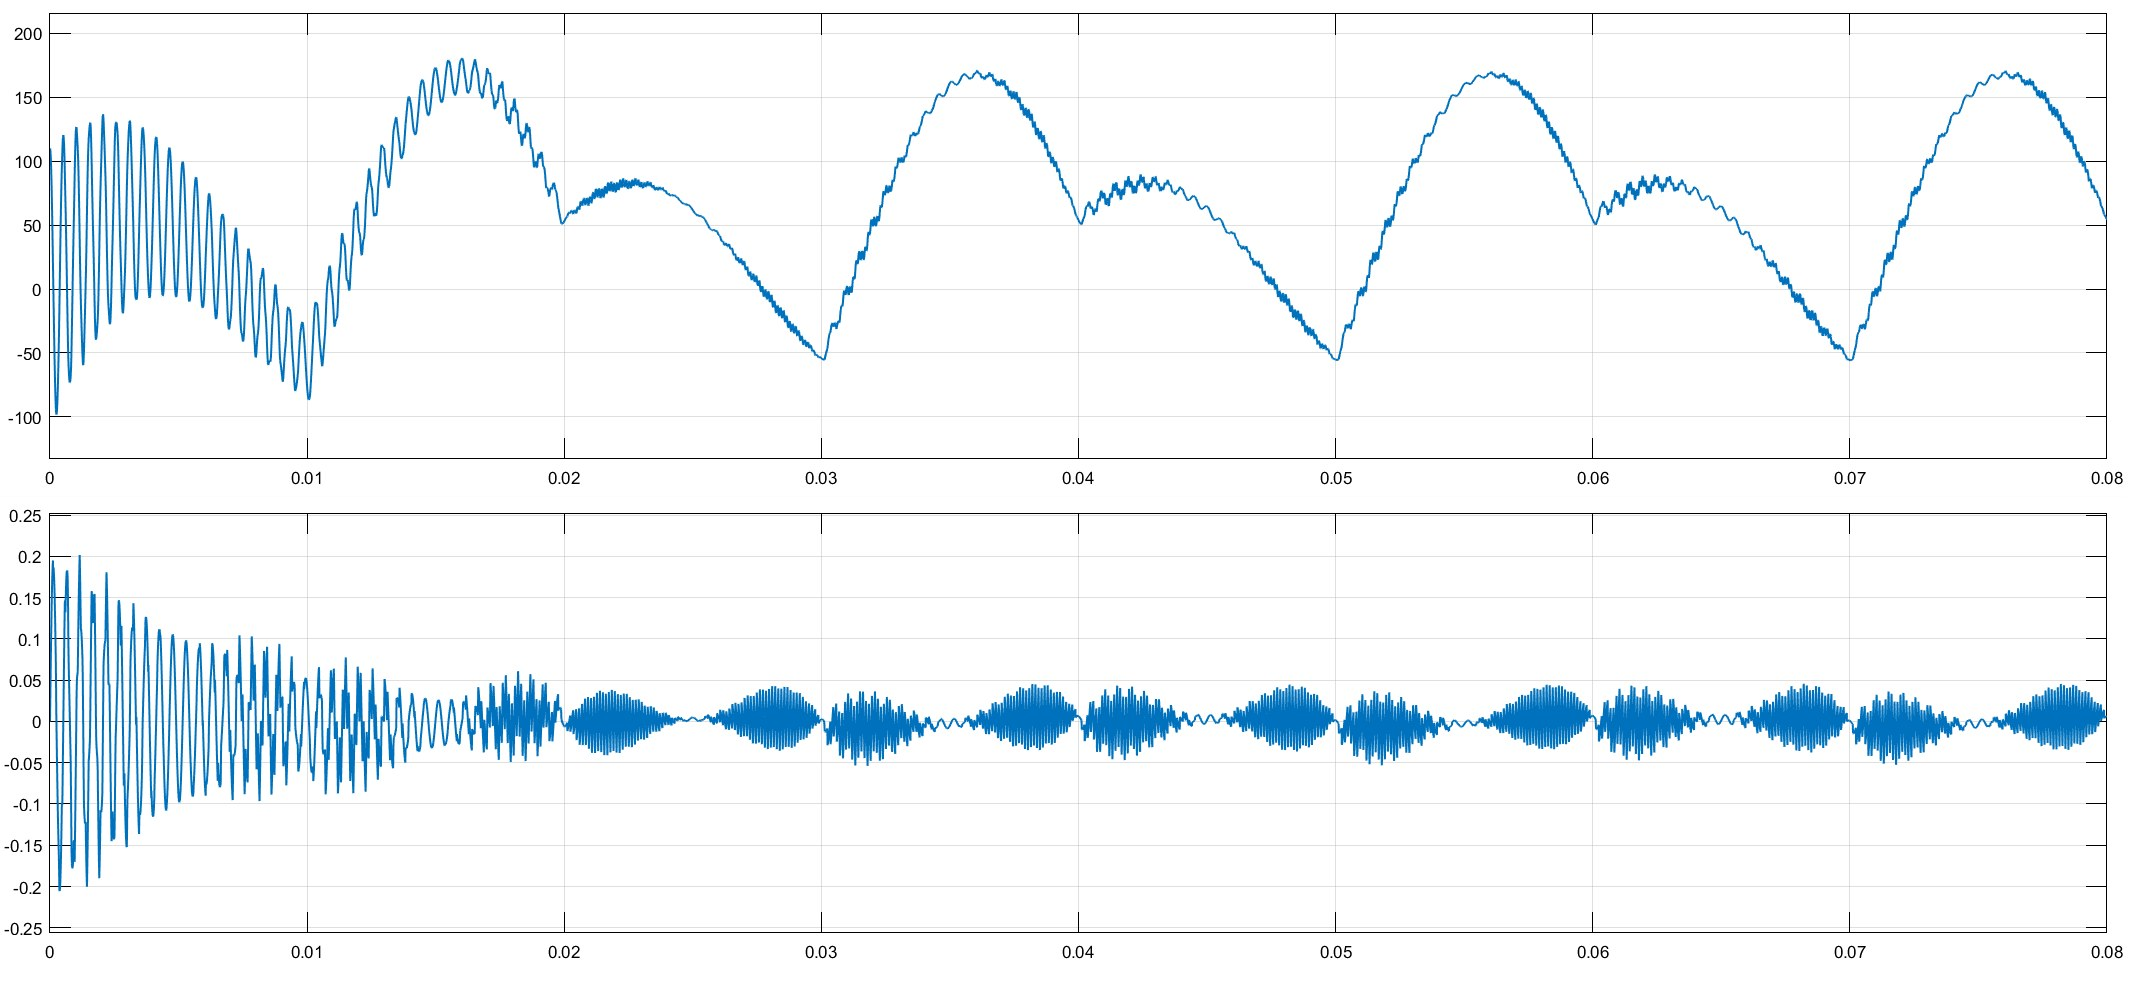
\includegraphics[width=\columnwidth]{figures/wave_h4_unipolar_cmv.jpg}
\caption{H4 with unipolar SPWM: (top) CMV in volts and (bottom) leakage current in amperes. The start-up transient decays within about two line cycles.}
\label{fig:wavesH4U}
\end{figure}

\subsection{H4 inverter with bipolar SPWM}
Fig.~\ref{fig:sweepH4B} shows the sweep from 1 to 40~kHz with $\Vdc=460$~V and $L=10$~mH. The leakage current is non-monotonic: there are strong peaks of about 500~mA at 2~kHz and about 440~mA at 12~kHz, a smaller peak of about 160~mA at 5~kHz, and a broad hump of about 120~mA near 25~kHz. For $\fsw\geq13$~kHz the leakage is in the range 20--60~mA up to 20~kHz and decreases to 14~mA at 40~kHz. The efficiency decreases from about 98.2\% at 1--2~kHz to 97.7\% at 15--40~kHz, with dips to 96.9\% at 6 and 10~kHz. The low-order THD is 33\% at 1~kHz, which is consistent with the large ripple at that frequency ($\Delta I_{pp,\max}\approx11.5$~A for $\Vdc=460$~V, $L=10$~mH, $\fsw=1$~kHz relative to a load-current amplitude of about 38~A), and falls below 0.2\% for $\fsw\geq5$~kHz. At 40~kHz the leakage current is 14~mA, the efficiency 97.72\% and the THD 0.10\% (Fig.~\ref{fig:fftH4B}).

The voltage across $\Cpv$ in this case (Fig.~\ref{fig:wavesH4B}) is a 50-Hz sinusoid between about 40 and 420~V, i.e., of amplitude about 190~V about a mean of $\Vdc/2=230$~V. This is half of the 384-V output amplitude and agrees with the effective source \eqref{eq:tcm}: even though the CMV of the bipolar bridge is constant on average, the grounded load terminal adds a term $-v_o/2$. Equation~\eqref{eq:floor} gives a line-frequency floor of 6.4~mA for this amplitude, below the 14~mA measured at 40~kHz.

\begin{figure}[!t]
\centering
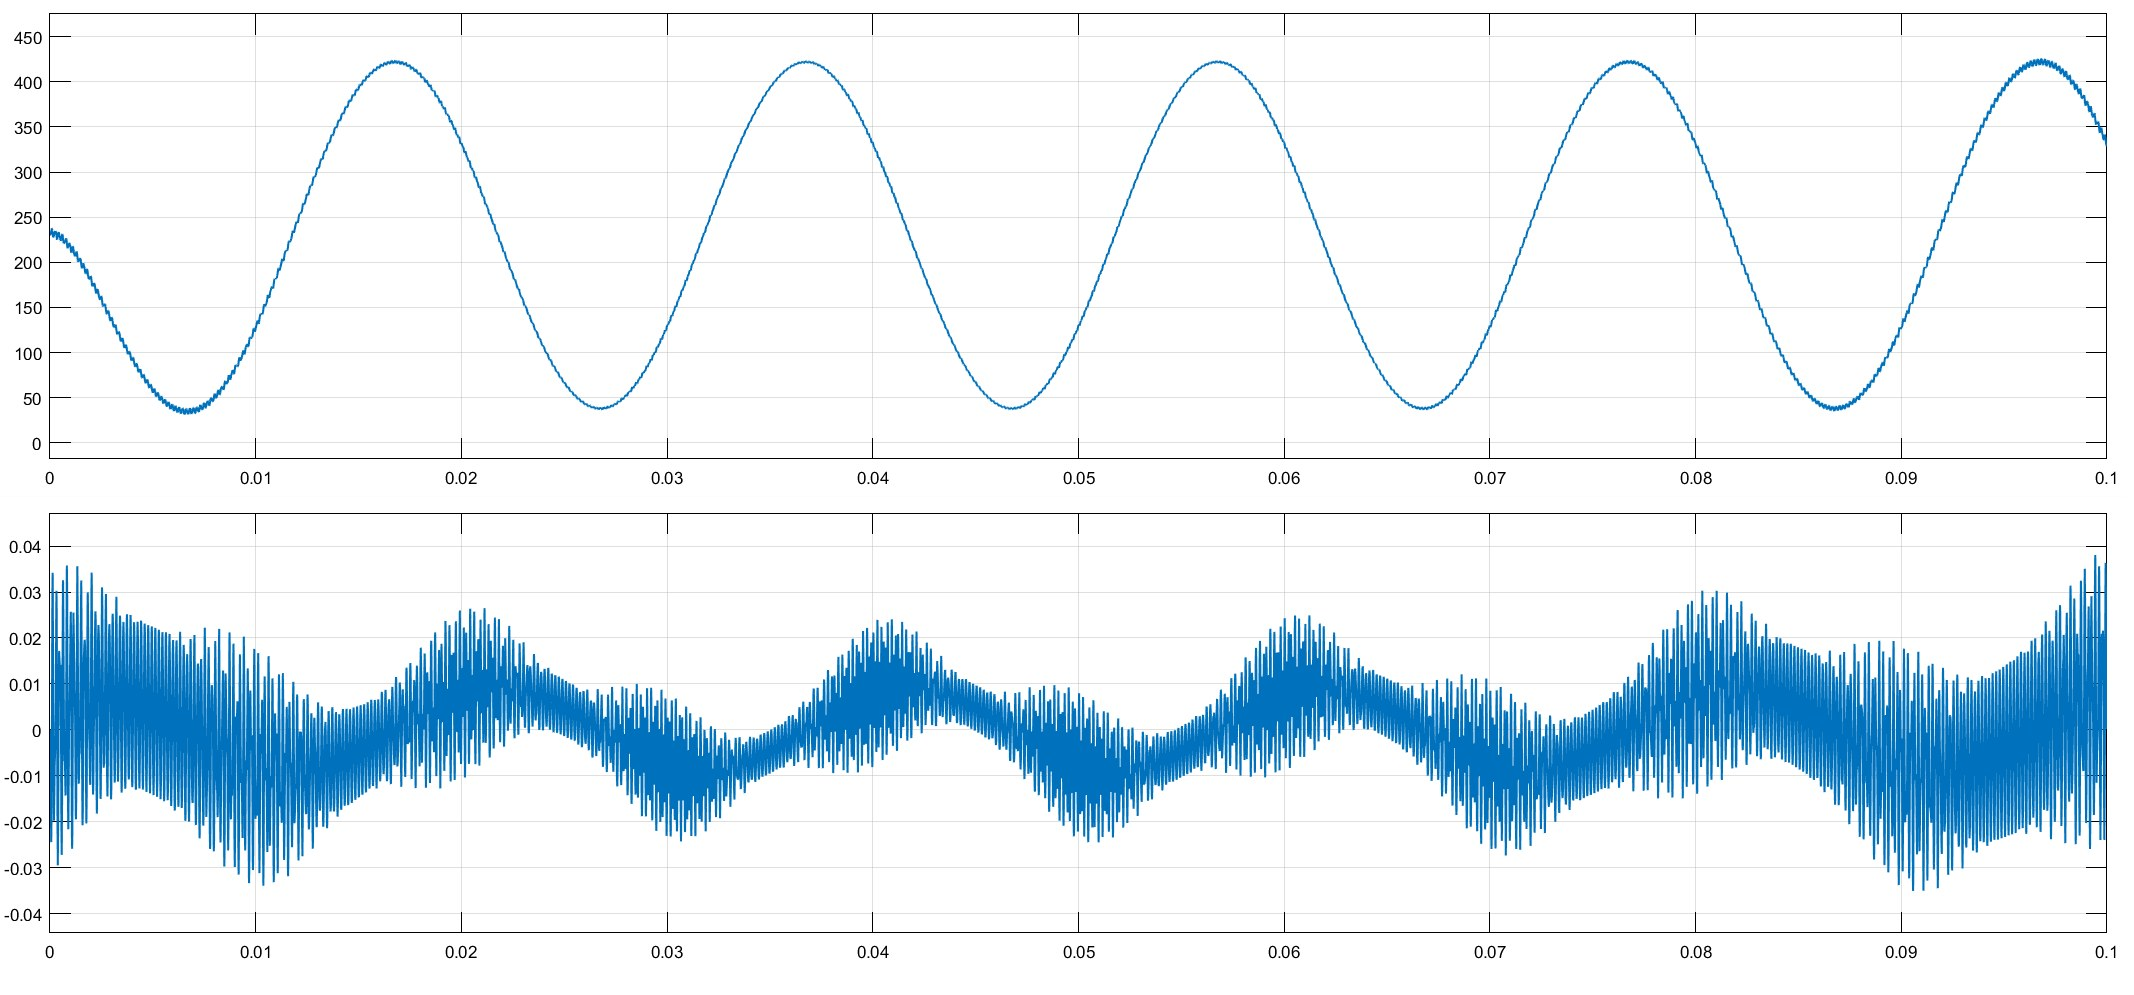
\includegraphics[width=\columnwidth]{figures/wave_h4_bipolar_cmv.jpg}
\caption{H4 with bipolar SPWM at the start of the simulation: (top) voltage across $\Cpv$ in volts and (bottom) leakage current in amperes.}
\label{fig:wavesH4B}
\end{figure}

Both major peaks fall at predicted frequencies, but by different mechanisms. The 2-kHz peak lies at $\fres/3=1.94$~kHz, so that $3\fsw\approx\fres$, as expected from the third harmonic of the carrier exciting the resonance. The 12-kHz peak lies at $2\fres=11.6$~kHz, which the mechanism of Section~\ref{sec:cm} does not predict, because it would require sub-harmonic content at $\fsw/2$ in the effective source. The smaller 5-kHz hump lies 14\% below $\fres$, which exceeds the 1-kHz sweep step; it is treated as a secondary feature that the first-order model does not explain (for example, a damping-related shift or an interaction with the DC-link and source impedance).

\begin{figure*}[!t]
\centering
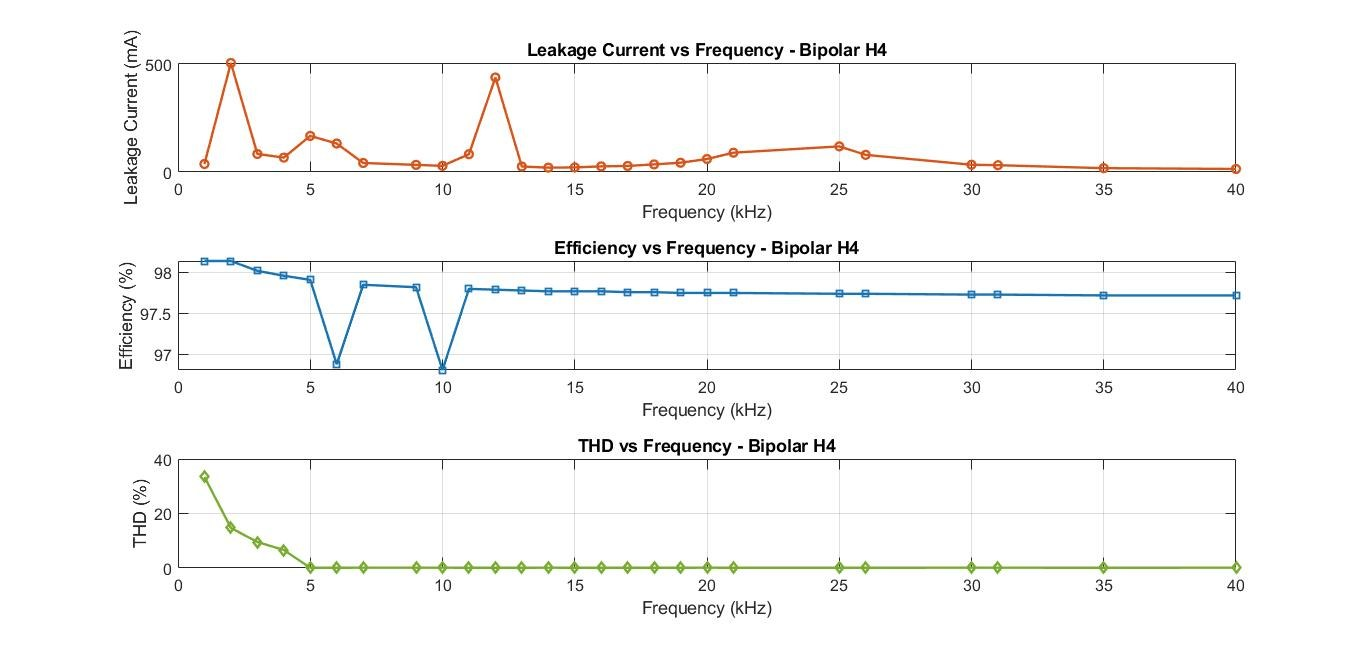
\includegraphics[width=0.85\textwidth]{figures/sweep_h4_bipolar.jpg}
\caption{H4 with bipolar SPWM: leakage current (mA), efficiency and THD versus switching frequency ($\Vdc=460$~V, $L_1=L_2=10$~mH, $R_L=10\;\Omega$, $\Cpv=150$~nF).}
\label{fig:sweepH4B}
\end{figure*}

\begin{figure}[!t]
\centering
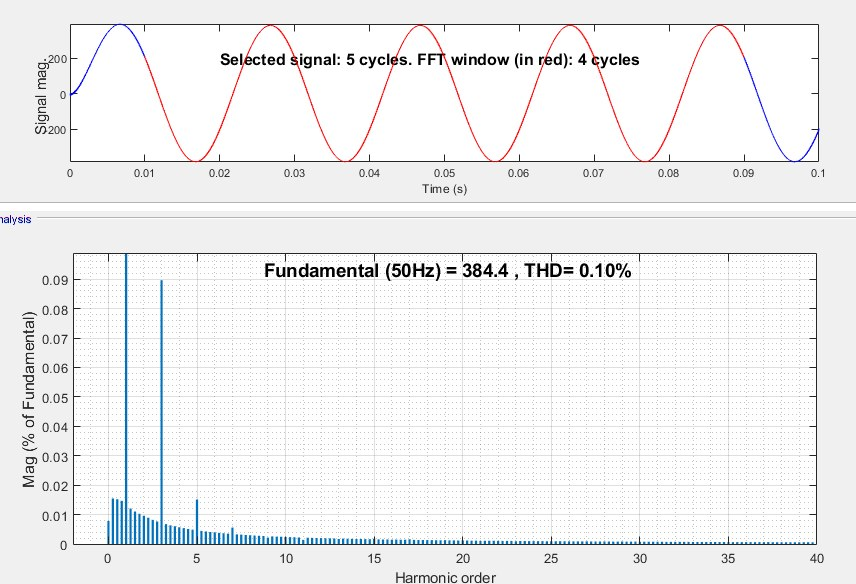
\includegraphics[width=\columnwidth]{figures/fft_h4_bipolar.jpg}
\caption{Powergui FFT of the H4 bipolar output voltage at 40~kHz: fundamental 384.4~V, THD $=0.10\%$ (harmonic orders up to 40; 5 simulated cycles, 4-cycle window).}
\label{fig:fftH4B}
\end{figure}

\subsection{Effect of the L filter on the output waveform}
Fig.~\ref{fig:h4out} shows the H4 unipolar output voltage before and after the filter. The unfiltered voltage is a three-level PWM waveform of $\pm220$~V; the filter removes the switching ripple and leaves a sinusoid with a start-up transient. The Powergui FFT, restricted to harmonic orders up to 40, gives a THD of 0.28\% before and 0.16\% after the filter. These numbers are small for both waveforms because the band covers only up to 2~kHz and therefore excludes the switching sidebands, which are the actual difference between the two waveforms. The low-order THD is thus a measure of the fundamental-band distortion (dead time, crossover, start-up transient), and the ripple attenuation of the filter is better evaluated from the waveform (Fig.~\ref{fig:h4out}) or from a wide-band FFT. A wide-band FFT, together with the compliance with the harmonic limits of \cite{IEEE519,IEEE1547} that depend on the short-circuit ratio of the point of connection, is part of the future work.

\begin{figure}[!t]
\centering
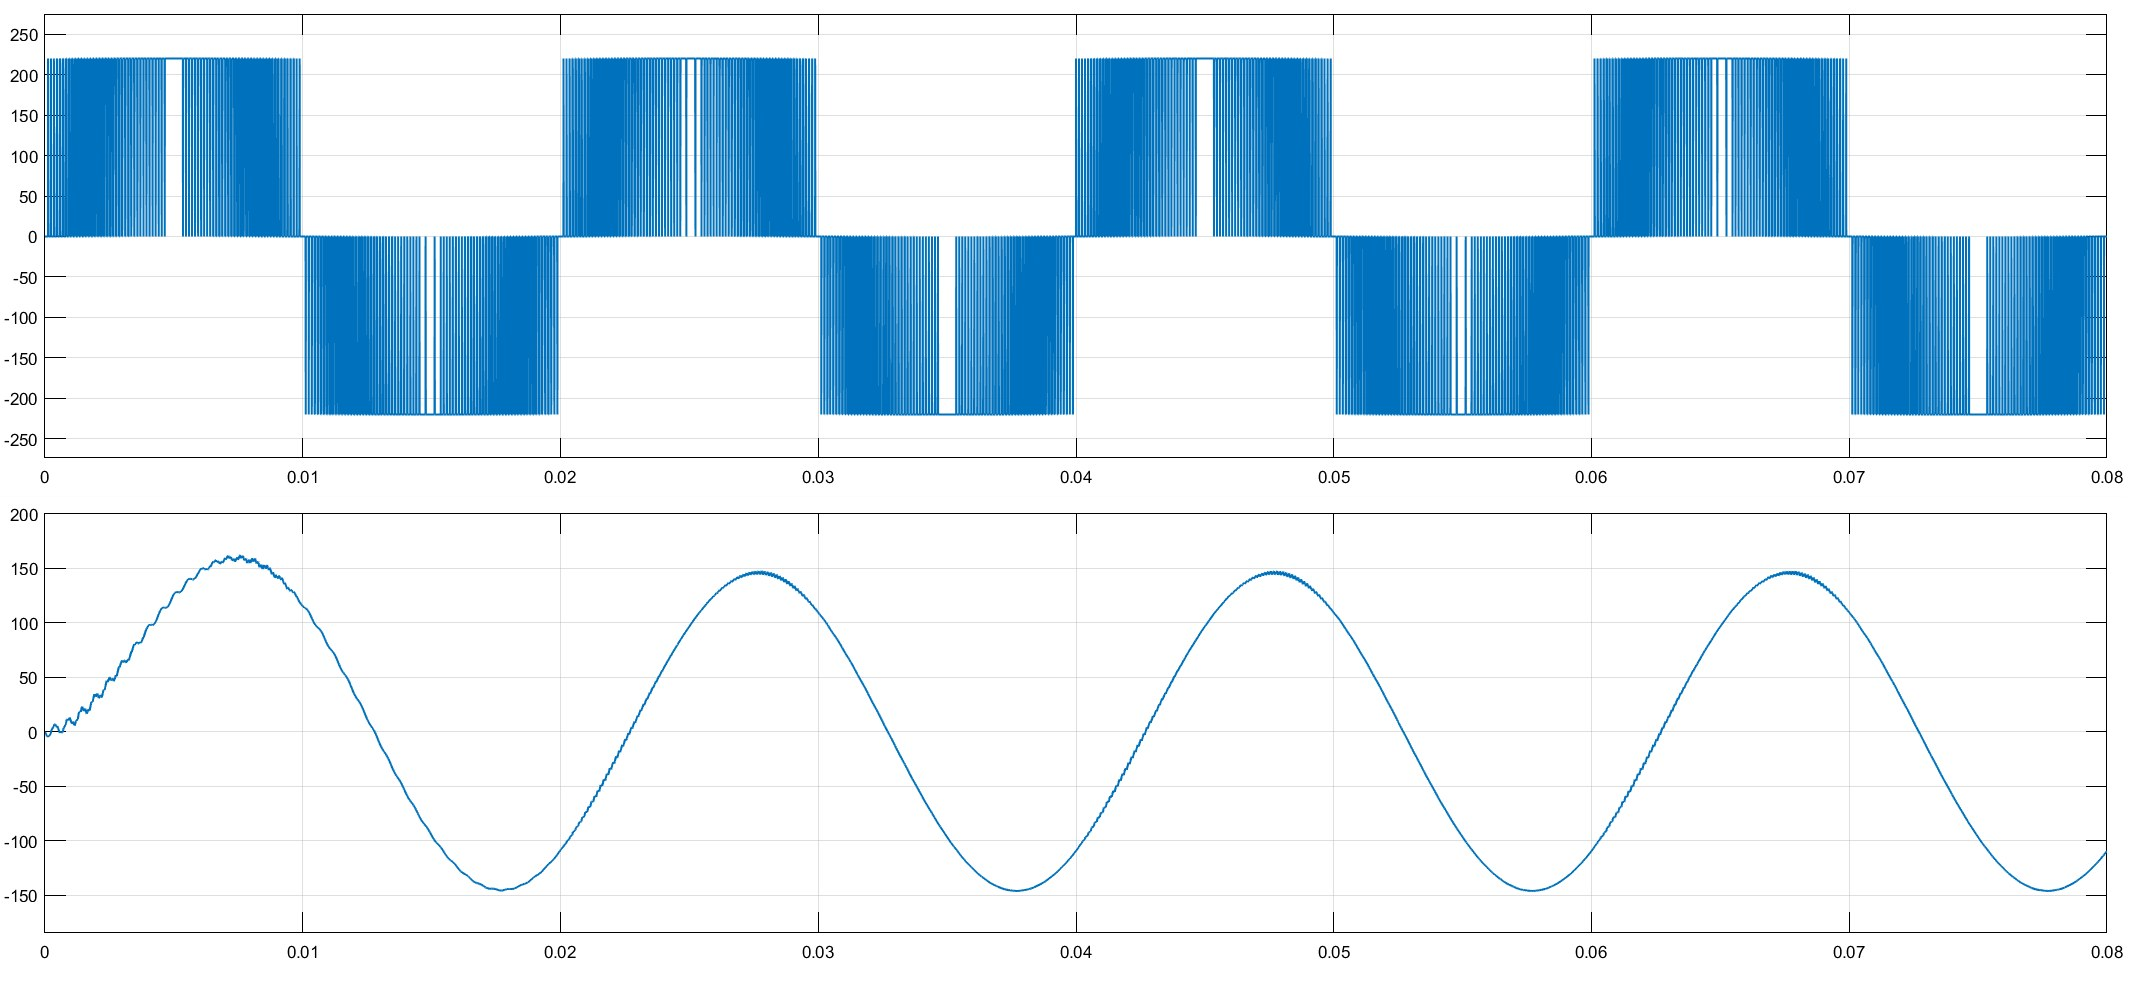
\includegraphics[width=\columnwidth]{figures/wave_h4_unipolar_out.jpg}
\caption{H4 with unipolar SPWM: (top) unfiltered and (bottom) filtered output voltage in volts ($\Vdc=220$~V, $L_1=L_2=90$~mH).}
\label{fig:h4out}
\end{figure}

\subsection{HERIC inverter with unipolar SPWM}
For HERIC with unipolar SPWM ($\Vdc=220$~V, $L=10$~mH, $R_L=10.68\;\Omega$) the sweep of 5--30~kHz in Fig.~\ref{fig:sweepHU} shows the most pronounced resonance of all cases: the leakage current rises from about 0.6~A at 5~kHz to a maximum of about 4~A at 6~kHz and falls steeply, to about 0.5~A at 7~kHz, and then more slowly to a few tens of milliamps above 20~kHz. The peak is within 3\% of the predicted $\fres=5.81$~kHz. At 26~kHz the leakage is 40.27~mA, the efficiency is 98.97\% and the low-order THD is 0.05\%. The efficiency is virtually independent of $\fsw$ (98.93--98.97\%, with a minimum at the resonance), and the THD increases only slightly from 0.05\% (up to about 16~kHz) to 0.09\% near 30~kHz. Fig.~\ref{fig:fftHU} shows the corresponding FFT. In this model the CMV is not constant: the CM and leakage waveforms (Fig.~\ref{fig:wavesHU}) display a 100-Hz rectified-sine envelope with high-frequency ripple, i.e., the AC bypass does not fully decouple the PV array during the zero-voltage interval; this is consistent with the leakage current of tens of mA at 26~kHz, an order of magnitude above the HERIC bipolar case. Keeping the leakage below 300~mA requires, from the plot, $\fsw\gtrsim9$~kHz.

\begin{figure}[!t]
\centering
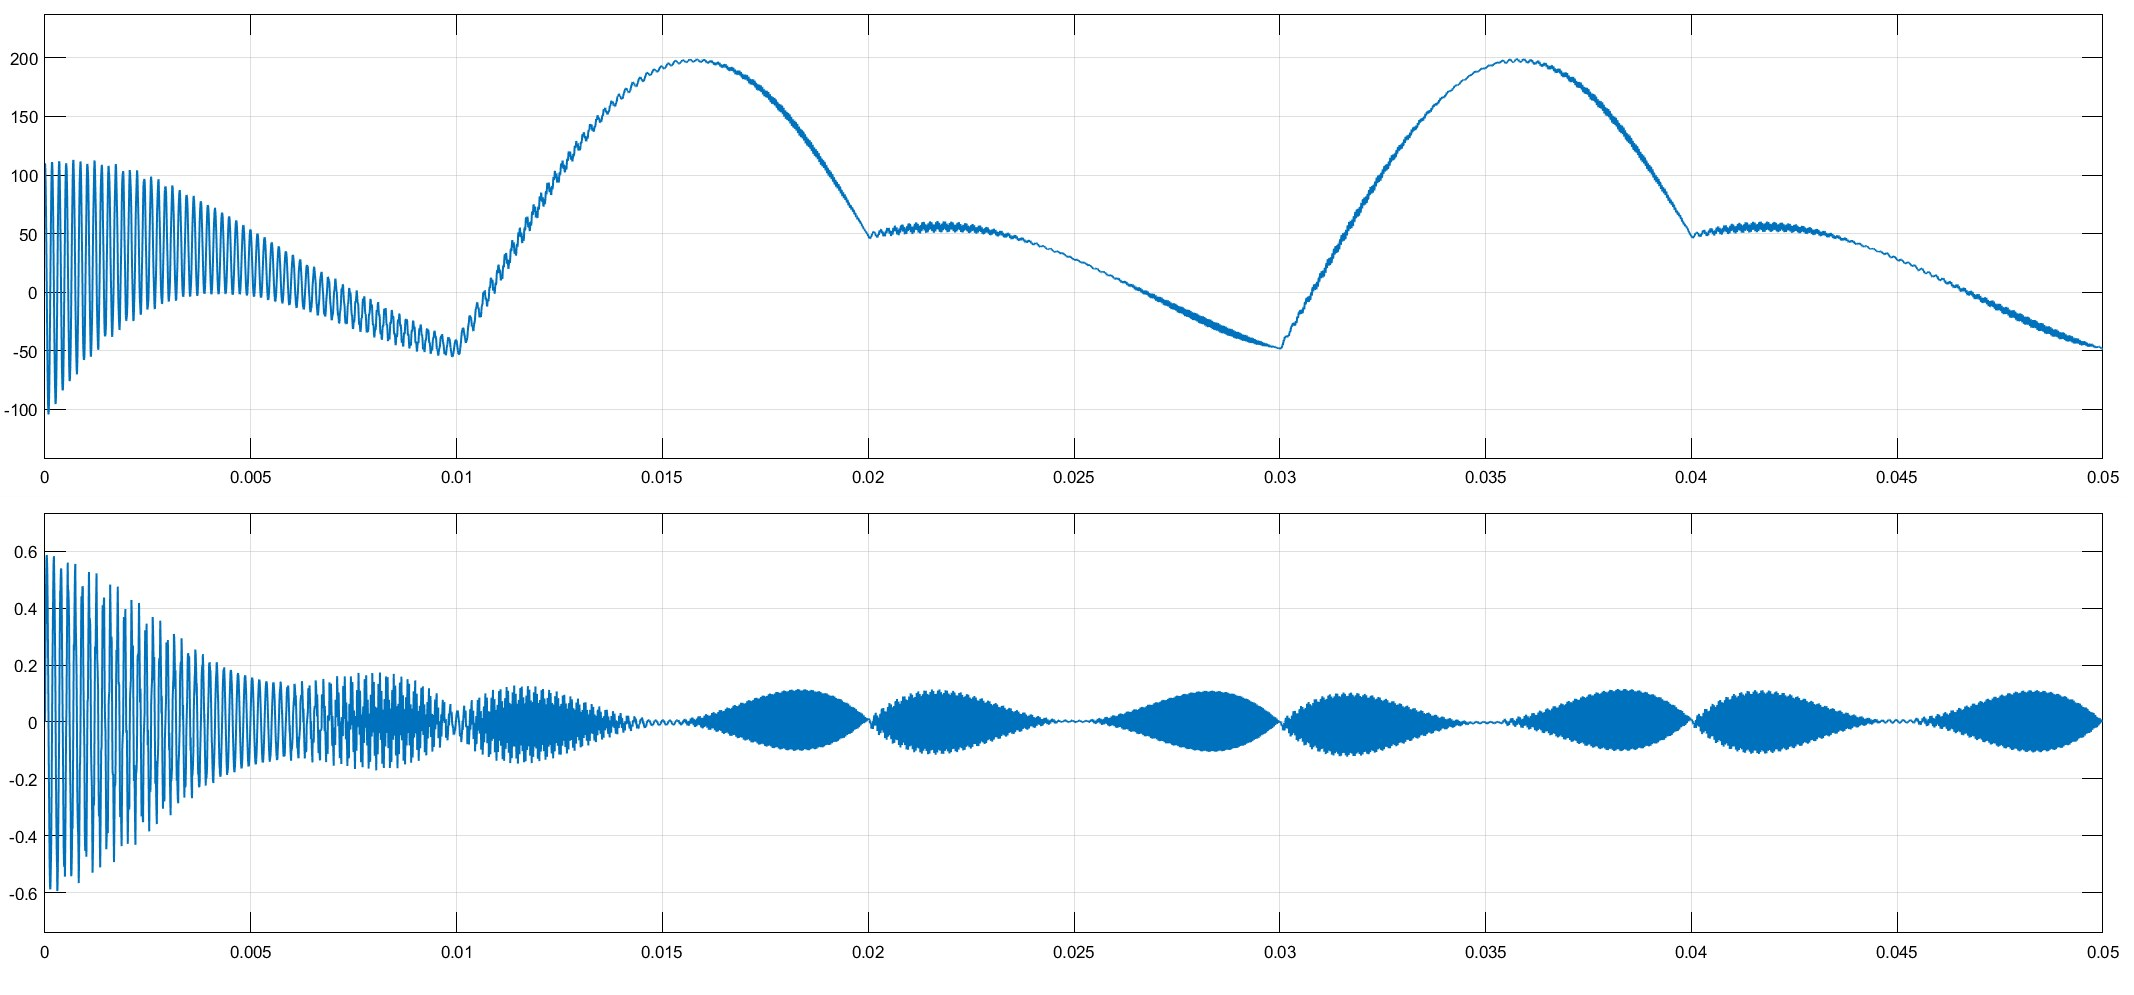
\includegraphics[width=\columnwidth]{figures/wave_heric_unipolar_cmv.jpg}
\caption{HERIC with unipolar SPWM: (top) voltage across $\Cpv$ in volts and (bottom) leakage current in amperes. The envelope repeats at 100~Hz, so the decoupling by the bypass is incomplete in the model.}
\label{fig:wavesHU}
\end{figure}

\begin{figure*}[!t]
\centering
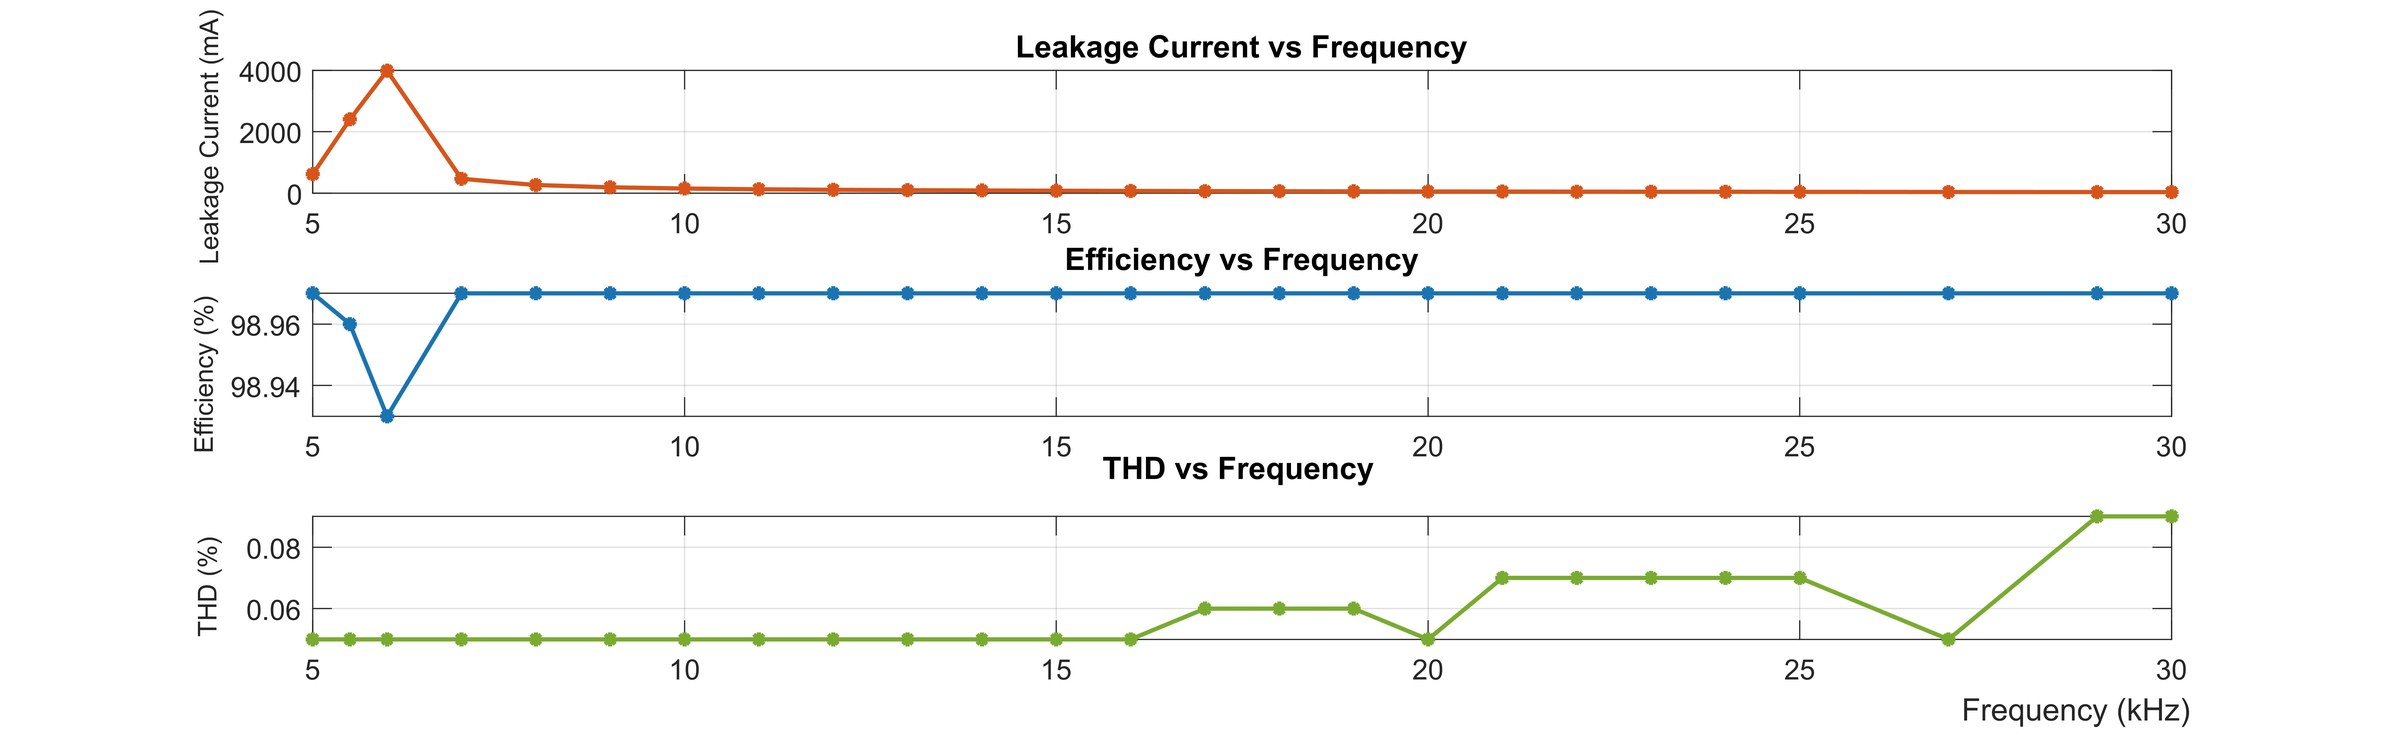
\includegraphics[width=0.85\textwidth]{figures/sweep_heric_unipolar.jpg}
\caption{HERIC with unipolar SPWM: leakage current (mA), efficiency and low-order THD versus switching frequency ($\Vdc=220$~V, $L_1=L_2=10$~mH, $R_L=10.68\;\Omega$, $\Cpv=150$~nF).}
\label{fig:sweepHU}
\end{figure*}

\begin{figure}[!t]
\centering
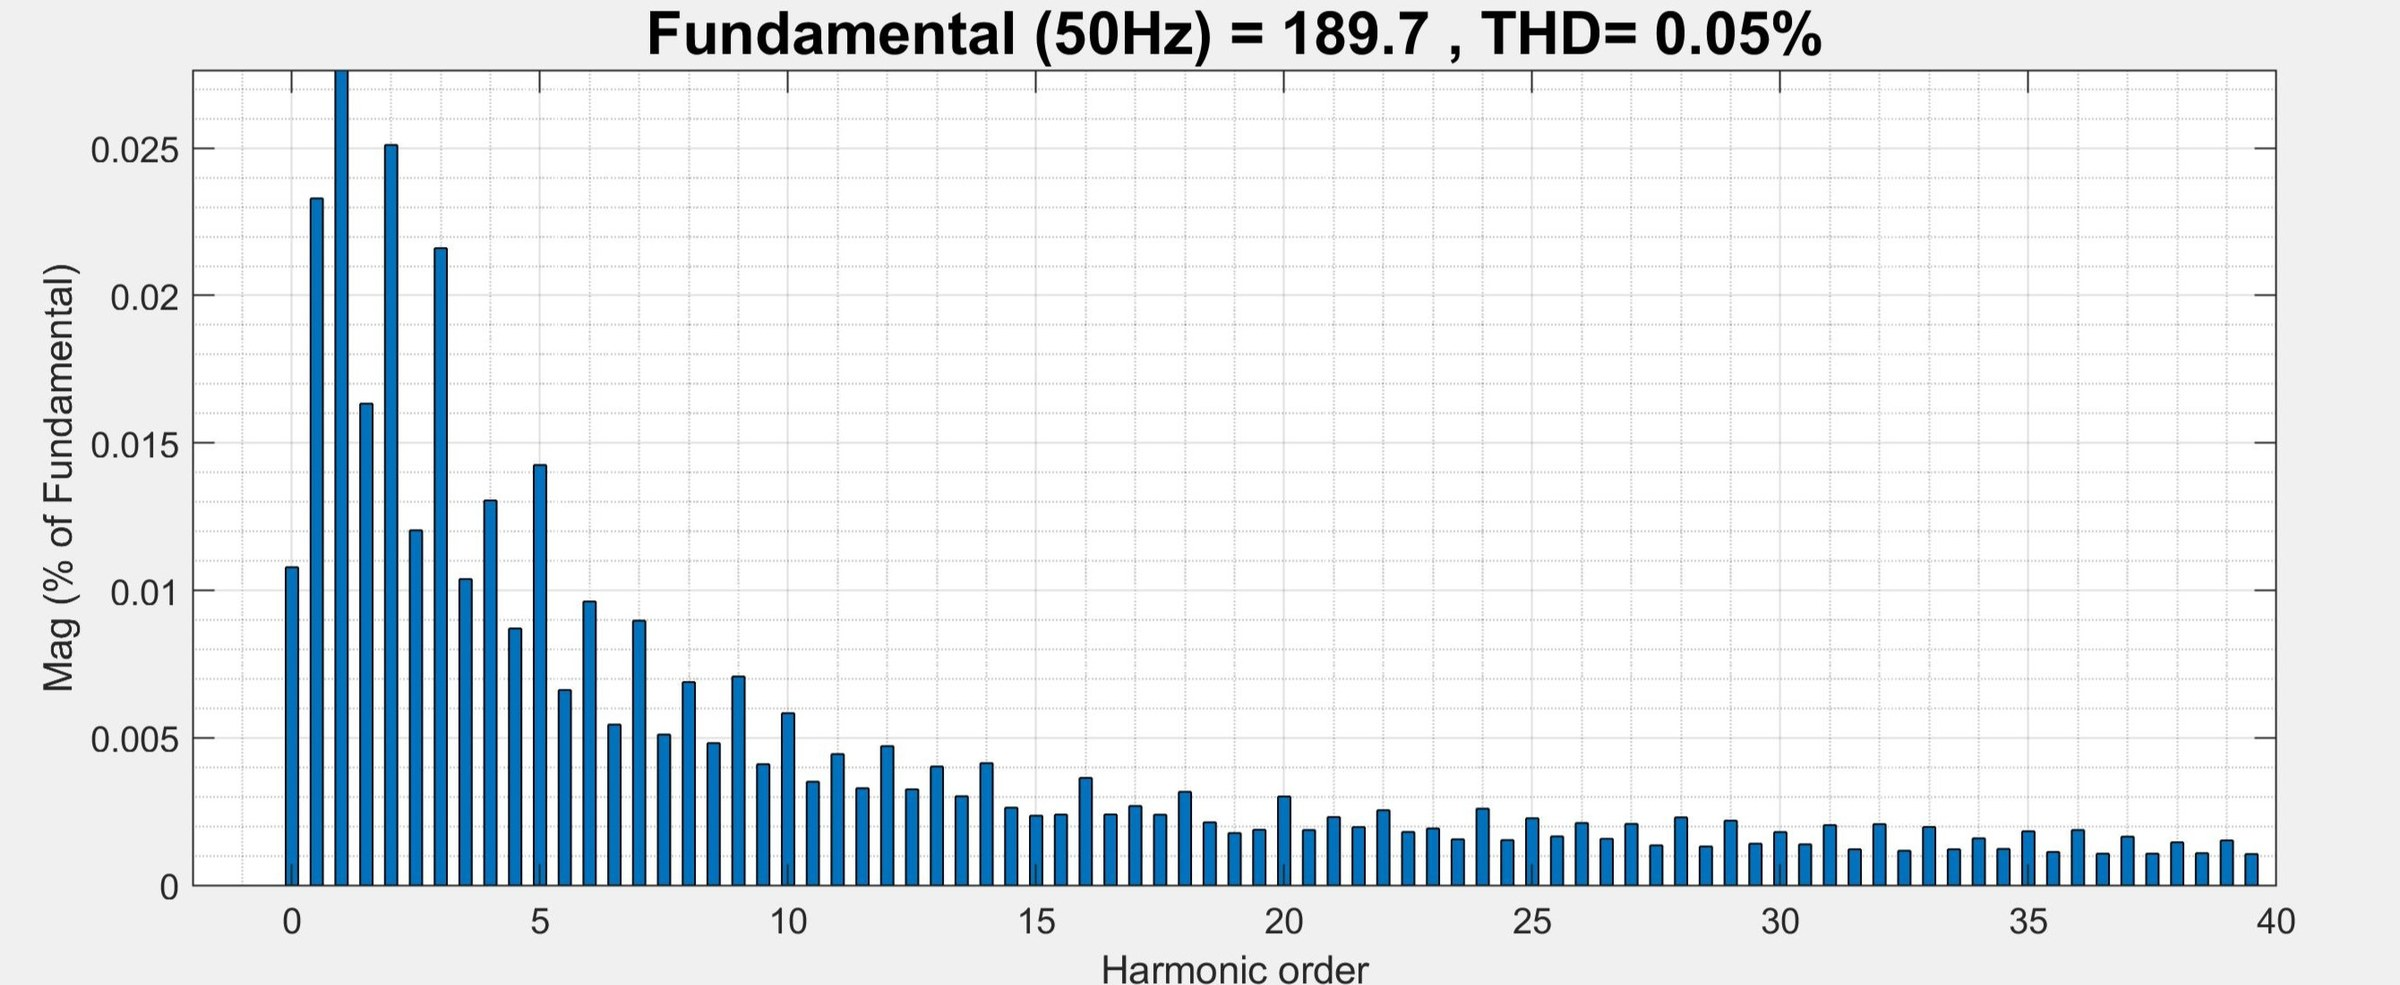
\includegraphics[width=\columnwidth]{figures/fft_heric_unipolar.jpg}
\caption{Powergui FFT of the HERIC unipolar output voltage with the filter: fundamental 189.7~V, THD $=0.05\%$ (harmonic orders up to 40).}
\label{fig:fftHU}
\end{figure}

\subsection{HERIC inverter with bipolar SPWM}
With bipolar SPWM and identical circuit parameters, the HERIC leakage current is much lower (Fig.~\ref{fig:sweepHB}): it has a modest maximum of about 15~mA at 5.5~kHz, which lies 5\% below the predicted $\fres$, falls to a minimum of about 3.2~mA at 10--10.5~kHz, and then rises slowly to about 5.5~mA at 35~kHz. At 13.5~kHz the leakage is 3.53~mA, and the low-order THD is 9.11\%. The leakage at the resonance is only about four times the floor, because the HF CMV content is small and the resonance has little to excite.

\begin{figure*}[!t]
\centering
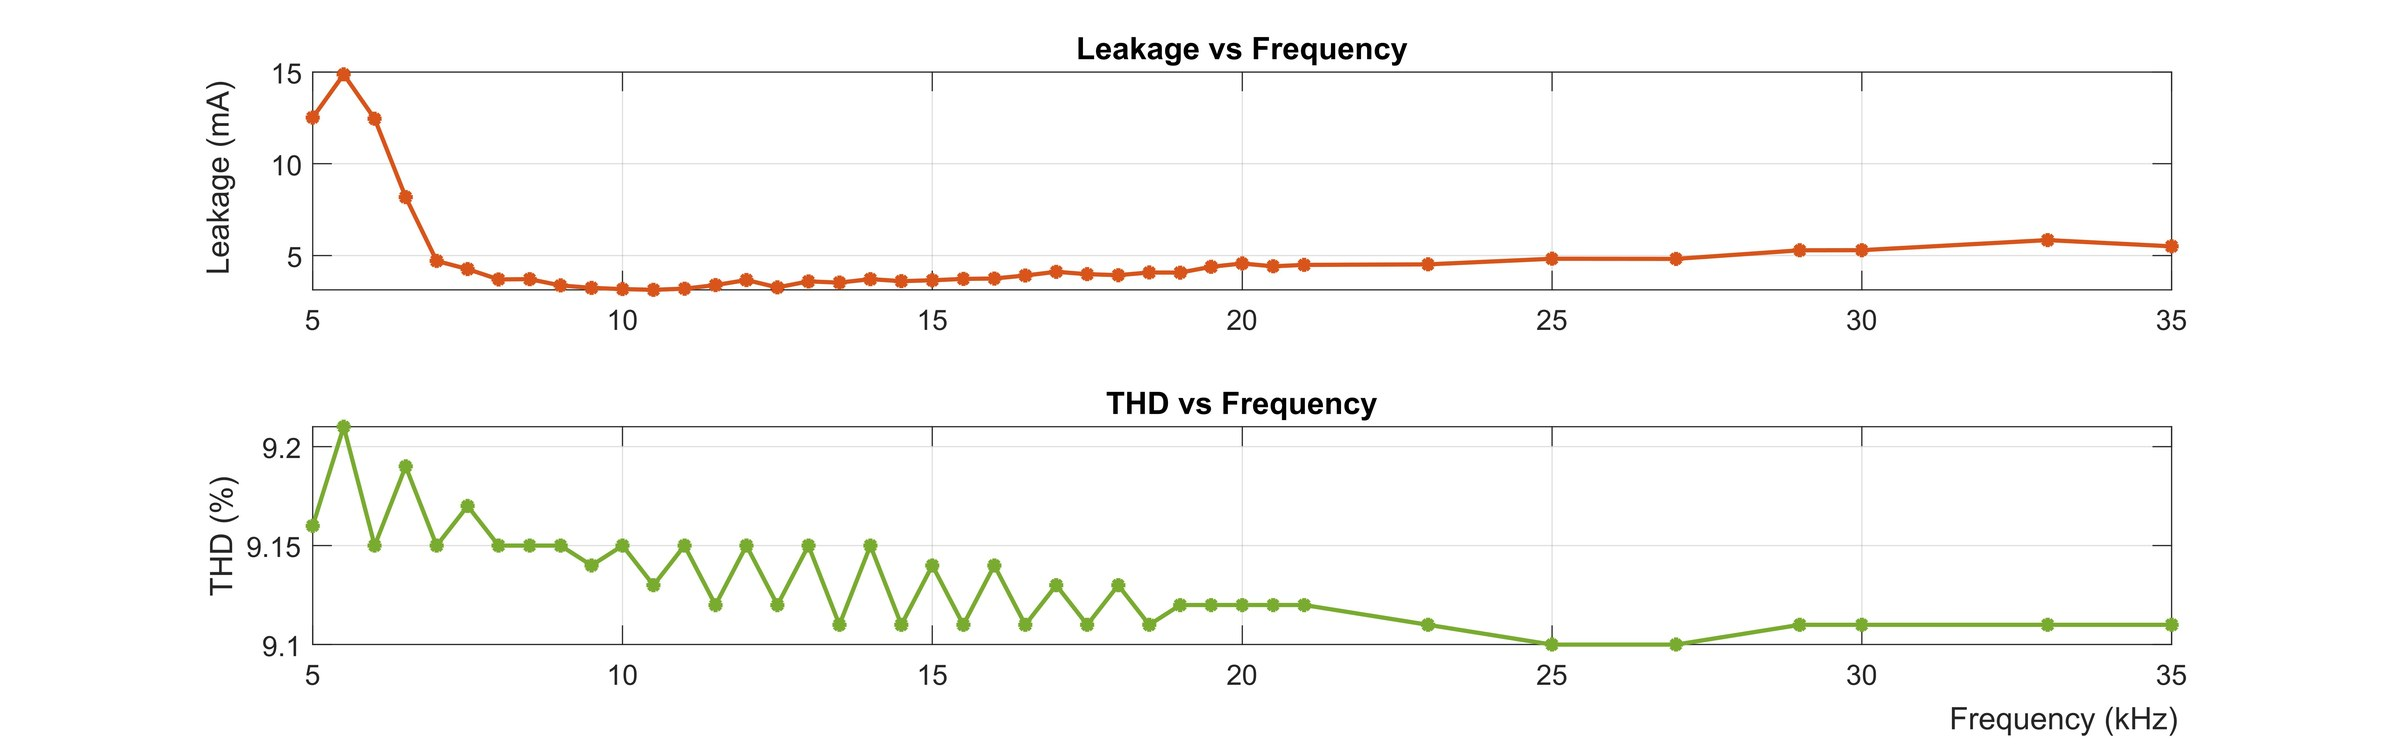
\includegraphics[width=0.85\textwidth]{figures/sweep_heric_bipolar.jpg}
\caption{HERIC with bipolar SPWM: leakage current (mA) and low-order THD versus switching frequency ($\Vdc=220$~V, $L_1=L_2=10$~mH, $R_L=10.68\;\Omega$, $\Cpv=150$~nF). An efficiency sweep was not recorded for this case.}
\label{fig:sweepHB}
\end{figure*}

\emph{Origin of the leakage floor.} The voltage across $\Cpv$ in this case (Fig.~\ref{fig:wavesHB}) is a smooth line-frequency waveform swinging between about 15 and 205~V, i.e., a 50-Hz component of about 95~V peak, which is half of the 190-V output amplitude, as \eqref{eq:tcm} predicts. Using~\eqref{eq:floor} with $V_{o,pk}=190$~V and $\Cpv=150$~nF gives $I_{\mathrm{floor}}\approx3.2$~mA, which matches the measured minimum of 3.2--3.5~mA. The leakage floor of this configuration is therefore the displacement current of the 50-Hz term of \eqref{eq:tcm} in $\Cpv$, not a switching-frequency effect, which explains why it is almost independent of $\fsw$ away from the resonance and implies that the bipolar HERIC configuration has essentially no carrier-frequency CMV in the simulation. (The 190-V amplitude is read from Fig.~\ref{fig:wavesHB}; the agreement should be regarded as an order-of-magnitude consistency check.) Table~\ref{tab:floor} applies the same estimate to the other cases: the line-frequency floor is 3--6~mA, so the leakage of 14--40~mA reported for the other three operating points is dominated by carrier-frequency components of $\vCM$. For H4 unipolar this is by design; for HERIC unipolar the bypass does not fully decouple the PV array in the model; for H4 bipolar the excess over the floor (about 8~mA at 40~kHz, and the large resonant peaks elsewhere) indicates a residual carrier-frequency CMV whose origin (switch parasitics, DC-source impedance or ripple asymmetry) was not isolated in this study.

\begin{table}[!t]
\renewcommand{\arraystretch}{1.2}
\caption{Line-frequency leakage floor from \eqref{eq:floor} versus reported operating points ($\Cpv=150$~nF)}
\label{tab:floor}
\centering
\footnotesize
\begin{adjustbox}{max width=\columnwidth}
\begin{tabular}{lcccc}
\toprule
Case & $V_{o,pk}$ (V) & $I_{\mathrm{floor}}$ (mA) & Operating point (kHz) & $I_{\mathrm{leak}}$ (mA) \\
\midrule
H4, unipolar & 220 & 3.7 & 8.5 & 15.4 \\
H4, bipolar & 384 & 6.4 & 40 & 14 \\
HERIC, unipolar & 190 & 3.2 & 26 & 40.3 \\
HERIC, bipolar & 190 & 3.2 & 13.5 & 3.5 \\
\bottomrule
\end{tabular}
\end{adjustbox}
\end{table}

\begin{figure}[!t]
\centering
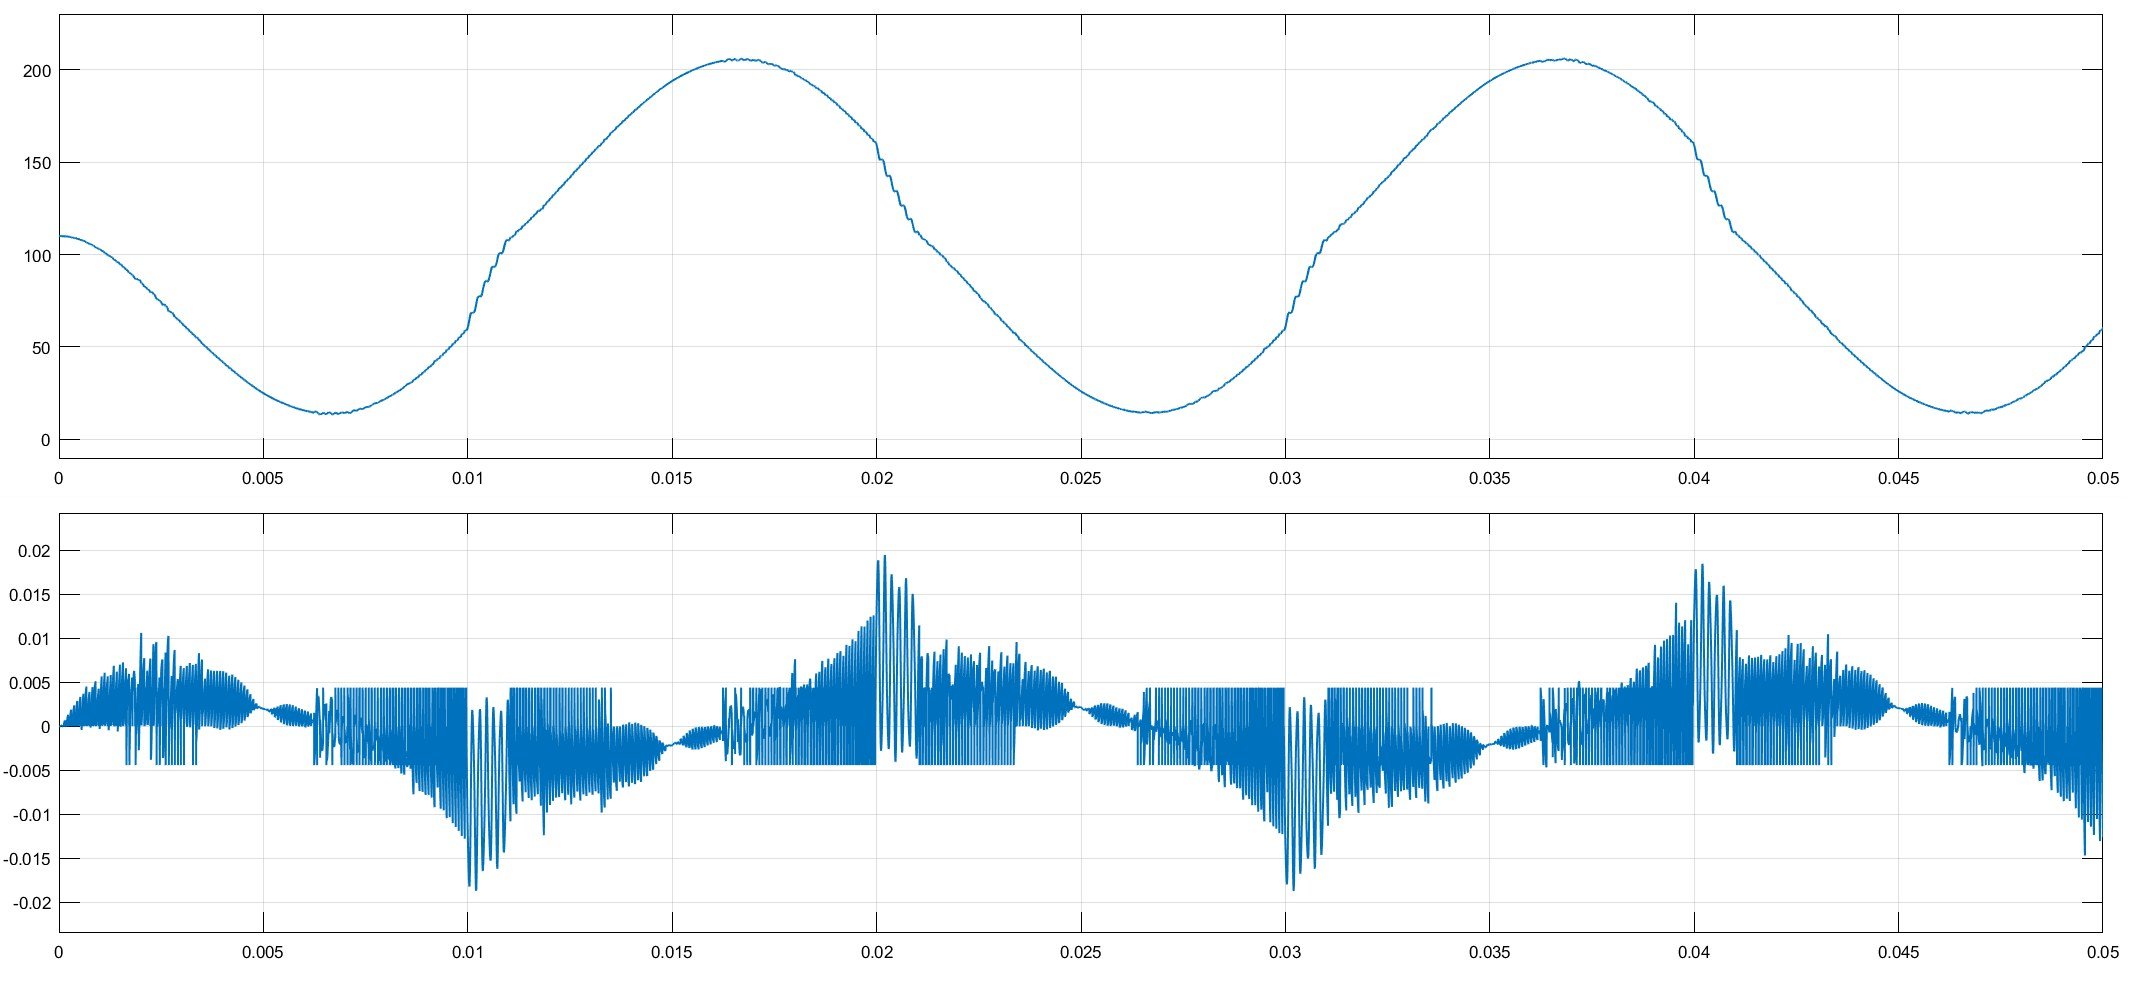
\includegraphics[width=\columnwidth]{figures/wave_heric_bipolar_cmv.jpg}
\caption{HERIC with bipolar SPWM: (top) CMV in volts and (bottom) leakage current in amperes.}
\label{fig:wavesHB}
\end{figure}

\emph{Origin of the THD.} The low-order THD of 9.1--9.2\% is almost constant over the entire sweep (5--35~kHz, Fig.~\ref{fig:sweepHB}). If it were caused by insufficient filtering of the switching ripple, it would decrease as $\fsw$ increases. Its invariance indicates a low-frequency origin. The filtered output voltage (Fig.~\ref{fig:outHB}) shows kinks at the zero crossings, i.e., crossover distortion, which is consistent with the interaction between the bipolar bridge modulation and the line-frequency bypass gating, and with the large DC component that was observed in the HERIC bipolar currents during the simulations. A correction of the bypass-gating synchronization, or the use of the conventional unipolar modulation, would be the first remedies to investigate; this has not been verified in the present work.

\begin{figure}[!t]
\centering
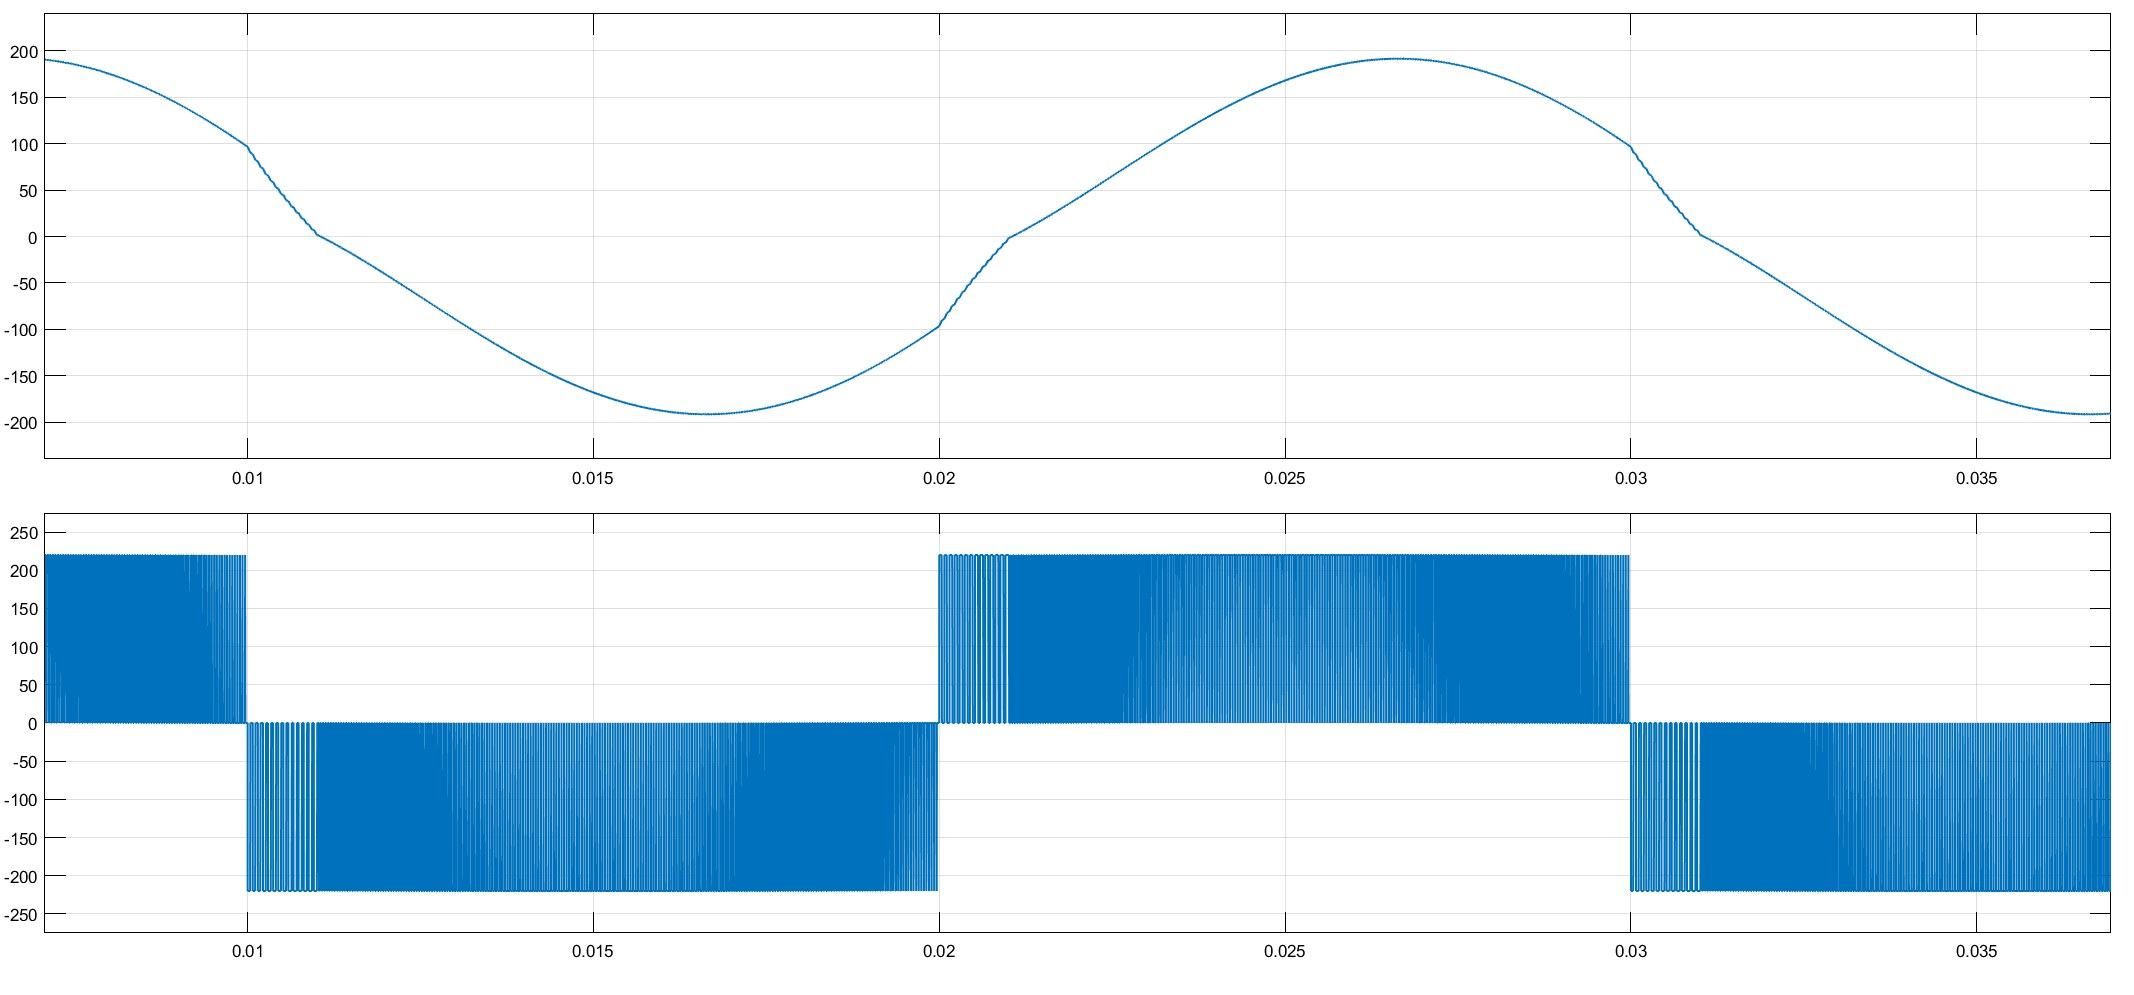
\includegraphics[width=\columnwidth]{figures/wave_heric_bipolar_out.jpg}
\caption{HERIC with bipolar SPWM: (top) filtered and (bottom) unfiltered output voltage. The kinks of the filtered voltage at the zero crossings (0.01~s, 0.02~s, 0.03~s) are the source of the roughly constant 9\% low-order THD.}
\label{fig:outHB}
\end{figure}

\subsection{CM-resonance analysis across cases}
Table~\ref{tab:res} compares the predicted resonance with the leakage peaks observed in the sweeps. The dominant peaks agree with $\fres$ (or $\fres/3$ and $2\fres$ for the H4 bipolar case) to within about 5\%, which is comparable to the sweep resolution of 0.5--1~kHz. The exception is the minor 5-kHz hump of the H4 bipolar case, which lies 14\% below $\fres$, outside the sweep resolution, and is therefore not explained by the first-order model (Section~\ref{sec:limits}). The agreement is not proof that the resonance mechanism is the only cause, but it is strong evidence, since the two values of $\Leq$ differ by a factor of nine and the peaks moved accordingly from about 2~kHz to about 6~kHz.

\begin{table}[!t]
\renewcommand{\arraystretch}{1.2}
\caption{Predicted CM resonance versus observed leakage peaks}
\label{tab:res}
\centering
\footnotesize
\begin{adjustbox}{max width=\columnwidth}
\begin{tabular}{lcccc}
\toprule
Case & Pred.\ $\fres$ (kHz) & Observed peak (kHz) & Relation & Deviation$^{e}$ (\%) \\
\midrule
H4, unipolar   & 1.94 & 2.0 & $\fsw=\fres$ & 3.1 \\
H4, bipolar (major) & 5.81 & 2.0 & $\fsw=\fres/3$ & 3.3 \\
H4, bipolar (major) & 5.81 & 12 & $\fsw=2\fres$ & 3.3 \\
H4, bipolar (minor) & 5.81 & 5 & $\fsw=\fres$ & 14 \\
HERIC, unipolar & 5.81 & 6.0 & $\fsw=\fres$ & 3.3 \\
HERIC, bipolar  & 5.81 & 5.5 & $\fsw=\fres$ & 5.3 \\
\bottomrule
\multicolumn{5}{p{0.95\columnwidth}}{\footnotesize $^{e}$Deviation $=|f_{\mathrm{peak}}-f_{\mathrm{pred}}|/f_{\mathrm{pred}}$, with $f_{\mathrm{pred}}$ the predicted frequency given in the Relation column ($\fres$, $\fres/3$ or $2\fres$), read from the sweep plots; the sweep step is 0.5--1~kHz.}
\end{tabular}
\end{adjustbox}
\end{table}

\emph{Frequency-selection rule.} A practical rule that follows from the results is to keep the switching frequency away from the resonance, from its sub-multiples and, as observed once, from twice its value: $0.8\fres<k\fsw<1.2\fres$ must be avoided for $k=1,2,3$, together with $1.6\fres<\fsw<2.4\fres$, and $\fsw>2.4\fres$ is preferable whenever the efficiency and the switching loss permit. For the H4 bipolar case ($\fres=5.81$~kHz) this excludes about 1.6--2.3~kHz, 2.3--3.5~kHz, 4.6--7~kHz and 9.3--14~kHz, which contain all three leakage peaks of this case (2, 5 and 12~kHz). The rule should be validated for other values of $\Cpv$ (the parasitic capacitance depends on humidity and surface conditions, which shifts $\fres$) and by measurement.

\subsection{Cross-topology comparison}
Table~\ref{tab:summary} summarizes the operating points of the four cases. Within the HERIC pair, which has identical parameters, bipolar SPWM leaks 3.53~mA versus 40.27~mA for unipolar SPWM, a ratio of about 11 at the respective operating points (about 8 at 26~kHz for which both curves are available), but at the cost of a THD of 9.11\% versus 0.05\%.

The H4 and HERIC cases were simulated with different DC voltages, filter inductances and load resistances (Table~\ref{tab:params}), so the estimated output power ranges from about 0.5~kW to 7.4~kW. Consequently, the leakage, efficiency and THD of H4 and HERIC in Table~\ref{tab:summary} should not be used to rank the topologies in absolute terms. For example, the H4 bipolar leakage (14~mA at 40~kHz) and the HERIC bipolar leakage (3.53~mA) differ in $\Vdc$ by a factor of 2.1 and in power by a factor of more than four. Within each case, however, the dependence on the switching frequency is a clean single-factor experiment. A common-parameter re-simulation is needed for a topology ranking and is planned.

\begin{table*}[!t]
\renewcommand{\arraystretch}{1.2}
\caption{Selected operating points and extremes (simulation)}
\label{tab:summary}
\centering
\footnotesize
\setlength{\tabcolsep}{3.5pt}
\begin{adjustbox}{max width=\textwidth}
\begin{tabular}{lcccccc}
\toprule
Case & Point & $I_{\mathrm{leak}}$ & $\eta$ & THD & Worst & Compliant \\
 & (kHz) & (mA) & (\%) & (\%) & peak (mA)$^{a}$ & from (kHz)$^{a}$ \\
\midrule
H4, unipolar & 8.5 & 15.4 & 97.18 & 0.16 & $\approx$750 @ 2 & $\ge 3$ \\
H4, bipolar & 40 & 14 & 97.72 & 0.10 & $\approx$500 @ 2 & see text \\
HERIC, unipolar & 26 & 40.27 & 98.97 & 0.05 & $\approx$4000 @ 6 & $\gtrsim 9$ \\
HERIC, bipolar & 13.5 & 3.53 & n/a & 9.11 & $\approx$15 @ 5.5 & all \\
\bottomrule
\end{tabular}
\end{adjustbox}\\[2pt]
\begin{minipage}{0.97\textwidth}\footnotesize
$^{a}$Read from the sweep figures; ``compliant'' means RMS leakage $<300$~mA. For H4 bipolar the leakage exceeds 300~mA near 2 and 12~kHz.
\end{minipage}
\end{table*}

%% Section 7: Discussion
\section{Discussion}
\label{sec:discussion}

\subsection{What the sweeps show}
The three mechanisms identified in the preceding sections can be separated by their dependence on the switching frequency. The first is the \emph{line-frequency floor} \eqref{eq:floor}, which is independent of $\fsw$ and of the topology, and which scales with $\Cpv$ and with the output voltage; it sets a lower bound of a few milliamperes for a 150-nF array (Table~\ref{tab:floor}). The second is the \emph{carrier-frequency component} of $\vCM$, which exists for H4 with unipolar SPWM by construction and for the imperfectly decoupled HERIC case in the simulation; it adds to the floor and falls with $1/f$ above resonance. The third is the \emph{resonance}, which multiplies whichever carrier-frequency content exists when $k\fsw\approx\fres$. The distinction is useful because only the third can be removed without changing the topology or the modulation, simply by choosing $\fsw$ and the filter inductance.

\subsection{Relation to topology-centered studies}
Reviews and comparisons of transformerless topologies conclude that decoupling or clamping the common-mode voltage reduces leakage relative to a conventional H4 inverter with unipolar modulation \cite{Li2015,Khan2020,Kolodziejski2023}, and comparative simulations are usually reported at a fixed switching frequency \cite{Kibria2023,Shrestha2025}. The present results do not contradict this: in the HERIC bipolar case the leakage floor is 3.5~mA, lower than any other case. However, they indicate that the leakage observed for a given topology at a fixed $\fsw$ depends on where that $\fsw$ lies relative to the CM resonance of the particular filter and parasitic capacitance. A fixed-frequency comparison can therefore overstate or understate the difference between topologies by one to two orders of magnitude (Figs.~\ref{fig:sweepH4U}--\ref{fig:sweepHB}), which is one more reason to compare topologies with identical filters and over a frequency range. The conclusion of \cite{Shrestha2025} that H5 gives the best balance between leakage, THD and efficiency is not tested here because H5 was not simulated.

\subsection{Trade-offs for the HERIC bipolar variant}
The bipolar HERIC configuration trades a very low leakage current for a poor low-order waveform quality: its 9.1\% THD is above the few-percent distortion levels typically applied to grid-connected equipment \cite{IEEE519,IEEE1547}, and the observed kinks at the zero crossings are compatible with a mismatch between the bridge modulation and the bypass gating. This variant is not recommended in the present form. Two routes are worth investigating: re-synchronizing the bypass gating with the zero crossing of the reference, and using the conventional unipolar HERIC modulation with a filter and gating that suppress the residual carrier-frequency CMV. In the unipolar case, the leakage of 40~mA at 26~kHz and the sensitivity to resonance suggest that attention to the switch parasitics and to the timing of the bypass transitions would be rewarded.

\subsection{Compliance with the leakage limits}
Table~\ref{tab:limits} summarizes the leakage-current limits of IEC~62109-2 for transformerless inverters up to 30~kVA, as quoted in manufacturer documentation of the standard, together with the compliance of the simulated cases. Only the continuous limit can be checked from RMS sweeps. In all four cases the continuous limit of 300~mA is exceeded only in a narrow band around the resonance (H4 unipolar: at 2~kHz; H4 bipolar: near 2 and 12~kHz; HERIC unipolar: at 5--8~kHz); HERIC bipolar never exceeds it. The avoidance bands of Section~\ref{sec:design} indicate that, in these cases, the resonance can be avoided at the design stage by an appropriate choice of $\fsw$, provided that $\Cpv$ is known to within a factor of about two; the price is paid in efficiency at the upper end of the range, which is not captured by the present loss model.

\begin{table}[!t]
\renewcommand{\arraystretch}{1.2}
\caption{Residual-current limits for transformerless inverters up to 30~kVA (as summarized from IEC 62109-2 manufacturer documentation) and simulated compliance}
\label{tab:limits}
\centering
\footnotesize
\begin{adjustbox}{max width=\columnwidth}
\begin{tabular}{p{3.6cm}p{4.3cm}}
\toprule
Condition & Requirement \\
\midrule
Continuous residual current $>300$~mA & Disconnect within 0.3~s \\
Sudden change of 30~mA & Disconnect within 300~ms \\
Sudden change of 60~mA & Disconnect within 150~ms \\
Sudden change of 150~mA & Disconnect within 40~ms \\
\midrule
Simulated RMS leakage $>300$~mA & H4 uni.: near 2~kHz; H4 bi.: near 2, 12~kHz; HERIC uni.: 5--8~kHz; HERIC bi.: never \\
\bottomrule
\end{tabular}
\end{adjustbox}
\end{table}

%% Section 8: Sensitivity of the resonance and design guidelines
\section{Sensitivity of the Resonance and Design Guidelines}
\label{sec:design}

\subsection{Impedance of the CM loop}
Fig.~\ref{fig:sens}(a) plots $|Z_{CM}(f)|=|\omega\Leq-1/(\omega\Cpv)|$ for the two $\Leq$ values of Table~\ref{tab:params}. The impedance has a deep minimum at $\fres$; at this frequency only the (neglected) series resistance of the loop limits the current, which explains why the simulated resonant peaks of several amperes greatly exceed the leakage current in the off-resonance region. Above resonance the loop is inductive, $|Z_{CM}|\approx\omega\Leq$, and the leakage associated with a CMV component of given amplitude decreases with frequency as $1/f$ (compare \eqref{eq:icm}); this is the mechanism behind the monotonic decrease of leakage with $\fsw$ in the upper part of the H4 unipolar and HERIC unipolar sweeps. Below resonance the loop is capacitive and the current rises with frequency as $\omega\Cpv$.

\begin{figure*}[!t]
\centering
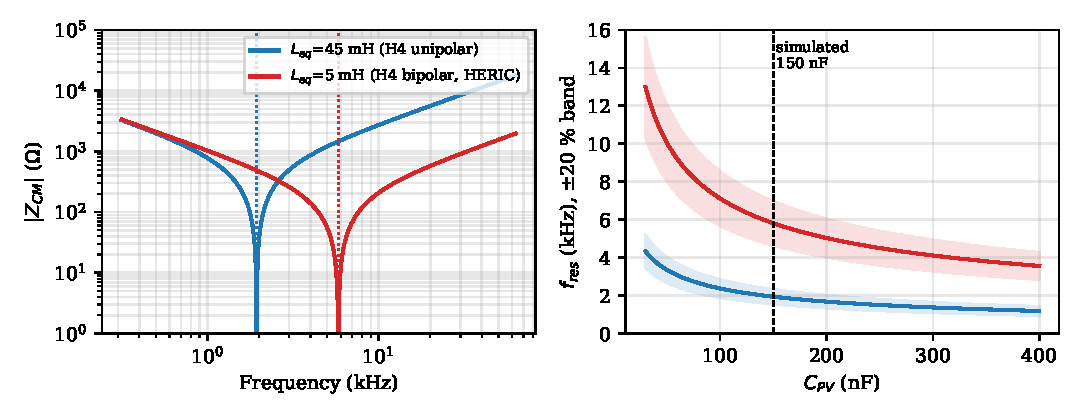
\includegraphics[width=0.85\textwidth]{figures/resonance_sensitivity.pdf}
\caption{Analytical CM-loop characteristics from \eqref{eq:icm} (no simulation data). (a)~Magnitude of the CM impedance for $\Cpv=150$~nF; dotted lines mark $\fres$. (b)~Resonance frequency versus parasitic capacitance, with the $\pm20\%$ avoidance band of the selection rule shaded.}
\label{fig:sens}
\end{figure*}

\subsection{Sensitivity to the parasitic capacitance}
The parasitic capacitance of a PV array is not a fixed number: it depends on the module technology, the mounting structure and the surface conditions, and increases when the module surface is wet \cite{Gubia2007,Khan2020}\todo{confirm that the cited sources give typical capacitance ranges before quoting numbers; none are quoted here}. Because $\fres\propto\Cpv^{-1/2}$, a doubling of $\Cpv$ lowers $\fres$ by 29\%. Table~\ref{tab:sens} lists the resonance for several values of $\Cpv$ together with the $\pm20\%$ avoidance bands for the two filter settings. The value of 330~nF is included only as a numerical example of a large capacitance.

\begin{table}[!t]
\renewcommand{\arraystretch}{1.2}
\caption{Resonance frequency and $\pm20\%$ avoidance band for varying $\Cpv$ (analytical, from \eqref{eq:icm})}
\label{tab:sens}
\centering
\footnotesize
\begin{adjustbox}{max width=\columnwidth}
\begin{tabular}{ccccc}
\toprule
 & \multicolumn{2}{c}{$\Leq=45$~mH} & \multicolumn{2}{c}{$\Leq=5$~mH} \\
\cmidrule(lr){2-3}\cmidrule(lr){4-5}
$\Cpv$ (nF) & $\fres$ (kHz) & Band (kHz) & $\fres$ (kHz) & Band (kHz) \\
\midrule
50  & 3.36 & 2.69--4.03 & 10.07 & 8.06--12.08 \\
100 & 2.37 & 1.90--2.84 & 7.12  & 5.70--8.54 \\
150 & 1.94 & 1.55--2.33 & 5.81  & 4.65--6.97 \\
300 & 1.37 & 1.10--1.64 & 4.11  & 3.29--4.93 \\
330 & 1.31 & 1.05--1.57 & 3.92  & 3.14--4.70 \\
\bottomrule
\end{tabular}
\end{adjustbox}
\end{table}

Two consequences follow. First, a switching frequency selected to avoid $\fres$ at 150~nF may fall into the avoidance band at a different capacitance: for the 5-mH filter, a design at $\fsw=7$~kHz is safe at 150~nF but is at the center of the band for 100~nF. The robust choice is $\fsw>2.4\fres$ evaluated for the \emph{smallest} expected $\Cpv$ (which gives the highest $\fres$); for $\Leq=5$~mH and $\Cpv=50$~nF this is $\fsw>24$~kHz. Second, a larger inductance moves $\fres$ down at the cost of a larger voltage drop: the 90-mH filter of the H4 unipolar case has $X_L/R_L>1$ (Table~\ref{tab:params}), which is much more than the 10\% rule of thumb for the voltage drop would permit, so the low $\fres$ of this case is partly a consequence of an oversized filter.

\subsection{Design procedure}
The results suggest the following procedure for selecting the switching frequency of a transformerless inverter with an L filter.
\begin{enumerate}
  \item Determine the bounds of $\Cpv$ for the installation (module technology, mounting, humidity), and compute $\fres$ from \eqref{eq:icm} at both bounds.
  \item Mark the avoidance bands $0.8\fres<k\fsw<1.2\fres$ for $k=1,2,3$ and $1.6\fres<\fsw<2.4\fres$ over the whole range of $\Cpv$.
  \item Choose $\fsw$ outside all bands and, if the efficiency target permits, above $2.4\fres$ evaluated at the smallest $\Cpv$.
  \item Verify with a time-domain simulation that the RMS leakage is below 300~mA and that the sudden changes of residual current remain below the steps of the standard \cite{IEC62109}; account for the effect of the switch output capacitances and dead time on the CMV.
  \item Check the efficiency and the filter ripple $\Delta I_{pp,\max}$ at the selected $\fsw$ with a loss model that includes the switching loss.
\end{enumerate}
Step~5 is essential: the sweeps in this paper do not capture the rise of the switching loss with $\fsw$, so the upper bound of the admissible frequency remains to be determined by a loss model or by measurement.

\subsection{Worked example}
Consider the H4 bipolar case ($L_1=L_2=10$~mH, $\Leq=5$~mH) installed on an array whose parasitic capacitance is expected to lie between 100~nF (dry) and 300~nF (wet). From Table~\ref{tab:sens}, $\fres$ lies between 4.11~kHz and 7.12~kHz, and the $\pm20\%$ bands on $\fsw$ for $k=1,2,3$ are $3.3$--$8.5$~kHz, $1.6$--$4.3$~kHz and $1.1$--$2.8$~kHz, respectively,
together with the band $6.6$--$17.1$~kHz around $2\fres$. Taken together over the range of $\Cpv$, these exclude $1.1~\text{kHz}<\fsw<17.1~\text{kHz}$, and the criterion $\fsw>2.4\fres$ at the smallest capacitance gives $\fsw>17.1$~kHz. The sweep of Fig.~\ref{fig:sweepH4B} (taken at 150~nF) shows that the leakage at 20 and 40~kHz is 60 and 14~mA, respectively, both well below the limit, and the choice between them is a matter of efficiency and ripple: 20~kHz has the lower switching loss but a ripple of $\Delta I_{pp,\max}=0.58$~A (about 1.5\% of the load-current amplitude), whereas 40~kHz reduces the ripple to 0.29~A. A design at 14~kHz, which the simple criterion $\fsw>2\fres$ would have allowed, falls inside the $2\fres$ band for the smallest-capacitance case and should be rejected. This example illustrates that the rule excludes a wide range for a poorly known $\Cpv$ and thus favors the upper part of the swept range or an inductance that places $\fres$ well below the intended $\fsw$.

\subsection{Experimental validation plan}
The results of this paper are simulation-based and the resonance rule should be validated on hardware before being relied upon. A minimal plan comprises (i) a single-phase H4/HERIC prototype in the 0.5--1~kW range with interchangeable L, LC and LCL filters and a selectable switching frequency; (ii) an emulated PV array in which a film capacitor bank of 50--330~nF is connected between the negative DC rail and the protective earth, replacing the unknown capacitance of real modules and allowing $\fres$ to be moved on purpose; (iii) measurement of $\iCM$ with a wide-band current probe in the earth lead and of the pole voltages, over the same frequency sweep as in simulation, with the RMS value compared with the 300~mA limit and the sudden steps with the limits of Table~\ref{tab:limits}; (iv) measurement of the efficiency with a power analyzer to bound the upper end of the admissible $\fsw$; and (v) an impedance measurement of the actual array (LCR meter between the shorted array terminals and the frame, dry and wet) to compare the measured $\Cpv$ with the assumed one. The comparison of the measured and predicted peak positions would directly test the first-order model \eqref{eq:icm}, whose neglect of loop resistance and of the ground-path inductance is the most important modeling assumption.

%% Section 9: Limitations
\section{Limitations}
\label{sec:limits}
The following limitations qualify the results.
\begin{enumerate}
  \item \emph{Simulation only.} No hardware validation is provided. The model is a resistive-load, open-loop model with a grounded load terminal and without a grid source, current controller or phase-locked loop; real systems include grid impedance and control, which change both the CM loop impedance and the modulation.
  \item \emph{Non-uniform parameters.} $\Vdc$, $L$ and $R_L$ differ between the H4 and HERIC cases, so a topology ranking is not supported (the cross-topology comparison above).
  \item \emph{Parasitic model.} The parasitic capacitance is a single 150~nF lumped capacitor; the resistive and inductive elements of the ground path, the switch output capacitances and dead time are not modeled, and these set the damping and the magnitude of the resonant peaks. The simulated peaks of several amperes are therefore an upper bound that highlights the resonance mechanism rather than a prediction of the magnitudes in a real system.
  \item \emph{Efficiency.} The efficiency does not include a complete switching-loss, core-loss or thermal model. The flat efficiency of the HERIC unipolar case indicates that the frequency dependence of switching loss is not captured. The efficiency values should be read as relative, conduction-dominated indicators.
  \item \emph{THD.} The THD is limited to harmonic orders up to 40 (2~kHz) and excludes the switching band; observation windows of 2--5 cycles include the residual start-up transient in some cases.
  \item \emph{HERIC bipolar.} The modulation used is not the conventional HERIC scheme, and the origin of its 9\% THD has been inferred, but not confirmed, from the waveforms.
  \item \emph{Filter sizing.} The series reactance of the filter is a large fraction of the load resistance (0.6--1.1, Table~\ref{tab:params}), so the inductances are larger than a 10\%-voltage-drop design would give. The magnitude of $\fres$, and hence the location of the leakage peaks, depends on this choice.
  \item \emph{Unexplained features.} The minor leakage peak of the H4 bipolar case at 5~kHz lies 14\% below the predicted resonance, and the 12-kHz peak lies at $2\fres$, where the carrier-harmonic mechanism predicts no peak; neither is explained by the first-order model. The $2.4\fres$ margin of the selection rule rests on this single observation.
  \item \emph{Sweep resolution.} The frequency step (0.5--1~kHz) limits the localization of the resonant peaks to about $\pm0.5$~kHz.
\end{enumerate}

%% Section 10: Conclusion
\section{Conclusion}
\label{sec:conclusion}
The leakage current of H4 and HERIC transformerless inverters with an L filter was investigated as a function of switching frequency (1--40~kHz) by simulation. In all four cases examined the leakage current exhibits sharp peaks, up to 0.75~A (H4 unipolar), 0.5~A (H4 bipolar) and 4~A (HERIC unipolar), located at the CM resonance $\fres=1/(2\pi\sqrt{\Leq\Cpv})$ at its low-order sub-multiples or, in one case, at twice its value, as predicted from the simulation parameters to within about 5\% for the dominant peaks. Away from the resonance, the leakage falls to 15.4~mA (H4 unipolar, 8.5~kHz), 14~mA (H4 bipolar, 40~kHz), 40.3~mA (HERIC unipolar, 26~kHz) and 3.5~mA (HERIC bipolar, 13.5~kHz). For identical parameters, the HERIC bipolar configuration yields about eleven times lower leakage than HERIC unipolar, with a floor that is consistent with the line-frequency term $v_o/2$ of the effective CM source acting on $\Cpv$, but a low-order THD of about 9.1\% that is independent of $\fsw$ and attributable to zero-crossing distortion. The practical consequence is a design rule: the switching frequency, its sub-multiples and twice $\fres$ should be placed outside a $\pm20\%$ band, and $\fsw>2.4\fres$ is preferable.

Future work comprises: (i) re-simulation of all topologies (including H5 and H6) with identical $\Vdc$, $L$, $R_L$ and power; (ii) inclusion of switching and thermal loss models and of the ground-path resistance; (iii) a grid-connected, closed-loop model with grid impedance; (iv) LC and LCL filters; (v) a correction of the HERIC bipolar gating; and (vi) a hardware prototype to validate the resonance-based frequency-selection rule for several values of $\Cpv$.


%% Elsevier declarations (required by Elsevier journals; placed after the Conclusion)
\section*{CRediT authorship contribution statement}
\textbf{Razowan Kabir}: Conceptualization, Methodology, Software, Investigation, Writing -- original draft, Visualization.
\textbf{Mridha Raju}: \todo{roles, answer my question below}.
\textbf{Mursida Khatun}: Formal analysis, Writing -- review \& editing.
\textbf{Pantho Mondal}: Software, Investigation, Writing -- review \& editing.
\textbf{Tanzim Khan}: Writing -- original draft, Writing -- review \& editing.
\textbf{Rabiul Islam}: Resources, Data curation, Writing -- review \& editing.
\textbf{A.T.M. Saiful Islam}: Supervision, Writing -- review \& editing.

\section*{Declaration of competing interest}
The authors declare that they have no known competing financial interests or personal relationships that could have appeared to influence the work reported in this paper.

\section*{Funding}
This research did not receive any specific grant from funding agencies in the public, commercial, or not-for-profit sectors.

\section*{Data availability}
The Simulink models, the switching-frequency sweep data (CSV files and the original Excel workbook) and the Python scripts used to analyse them are openly available in Zenodo at https://doi.org/\todo{10.5281/zenodo.XXXXXXX} (development repository: https://github.com/\todo{your-username}/h4-heric-leakage-current-resonance).

\section*{Declaration of generative AI and AI-assisted technologies in the writing process}
During the preparation of this work the authors used Claude (Anthropic) in order to help draft and edit the manuscript text, check the derivations and format the \LaTeX{} source. After using this tool, the authors reviewed and edited the content as needed and take full responsibility for the content of the publication.

\appendix
%% Appendix A: Derivation of the CM model
\section{Derivation of the CM Model}
\label{app:cm}
Consider the circuit of Fig.~\ref{fig:schematic} with $L_1=L_2=L$. Let $v_{QN}$ be the potential of the grounded node Q with respect to the negative DC rail $N$. Let $i_A$ be the current flowing from node A through $L_1$ and $R_L$ to Q, and $i_B$ the current flowing from node B through $L_2$ to Q. Kirchhoff's voltage law gives, for the two branches,
\begin{align}
v_{AN}-v_{QN}&=L\frac{di_A}{dt}+v_o, \label{eq:kvl1}\\
v_{BN}-v_{QN}&=L\frac{di_B}{dt}, \label{eq:kvl2}
\end{align}
where $v_o=R_Li_A$ is the load voltage (P with respect to Q). Adding \eqref{eq:kvl1} and \eqref{eq:kvl2} and using $\vCM=(v_{AN}+v_{BN})/2$,
\begin{equation}
2\vCM-v_o-2v_{QN}=L\frac{d(i_A+i_B)}{dt}.
\end{equation}
The sum $\iCM=i_A+i_B$ leaves node Q through the ground and returns to $N$ through $\Cpv$, so that $v_{QN}=\frac{1}{\Cpv}\int\iCM\,dt$. Therefore
\begin{equation}
\vCM-\frac{v_o}{2}=\frac{L}{2}\frac{d\iCM}{dt}+\frac{1}{\Cpv}\int\iCM\,dt,
\end{equation}
which is the series connection of $\Leq=L/2$ and $\Cpv$ driven by $e(t)=\vCM-v_o/2$. Taking the Laplace transform gives \eqref{eq:icm}. No assumption on $R_L$ has been made: the load enters only through $v_o$. In a grid-connected inverter the grounded neutral and the grid voltage play the roles of node Q and $v_o$, with the grid impedance neglected. The derivation is first-order: it neglects the resistance of the loop, the inductance and resistance of the ground path, and the switch output capacitances.

%% Appendix B: Operating modes and switching states
\section{Operating Modes and Switching States}
\label{app:modes}
Table~\ref{tab:modes} lists the ideal operating modes of the configurations, with the pole voltages, the resulting $\vCM$ and $\vDM$ according to \eqref{eq:cmdm}, and the conducting devices. For the H4 inverter with unipolar SPWM, modes~2 and~4 connect both output nodes to the same rail, so that $\vCM$ takes the values $\Vdc$ and $0$ in the two freewheeling states while taking $\Vdc/2$ in the active states. This variation of $\vCM$ at the carrier frequency is the source of the leakage current of the H4 unipolar case. In the HERIC inverter the freewheeling current circulates through the AC bypass, the bridge switches are all off, and the PV side is disconnected, so that the ideal $\vCM$ remains at $\Vdc/2$.

\begin{table}[!t]
\renewcommand{\arraystretch}{1.2}
\caption{Ideal operating modes ($V_{dc}$-normalized)}
\label{tab:modes}
\centering
\footnotesize
\setlength{\tabcolsep}{3pt}
\begin{adjustbox}{max width=\columnwidth}
\begin{tabular}{llcccc}
\toprule
Topology / mode & Conducting devices & $v_{AN}$ & $v_{BN}$ & $\vDM$ & $\vCM$ \\
\midrule
H4 unip.\ 1 (active $+$) & $S_1,S_4$ & $\Vdc$ & 0 & $\Vdc$ & $\Vdc/2$ \\
H4 unip.\ 2 (free.\ $+$) & $S_1$, $D_3$ & $\Vdc$ & $\Vdc$ & 0 & $\Vdc$ \\
H4 unip.\ 3 (active $-$) & $S_2,S_3$ & 0 & $\Vdc$ & $-\Vdc$ & $\Vdc/2$ \\
H4 unip.\ 4 (free.\ $-$) & $S_2$, $D_4$ & 0 & 0 & 0 & 0 \\
\midrule
HERIC 1 (active $+$) & $S_1,S_4$ & $\Vdc$ & 0 & $\Vdc$ & $\Vdc/2$ \\
HERIC 2 (free.\ $+$) & $S_5$ branch$^{d}$ & \multicolumn{2}{c}{floating} & 0 & $\Vdc/2$ \\
HERIC 3 (active $-$) & $S_2,S_3$ & 0 & $\Vdc$ & $-\Vdc$ & $\Vdc/2$ \\
HERIC 4 (free.\ $-$) & $S_6$ branch$^{d}$ & \multicolumn{2}{c}{floating} & 0 & $\Vdc/2$ \\
\bottomrule
\multicolumn{6}{p{0.9\columnwidth}}{\footnotesize $^{d}$The thesis labels the bypass for the positive half-cycle as $S_6$ and for the negative half-cycle as $S_5$; \todo{make the labelling of $S_5$/$S_6$ in the text, Fig.~\ref{fig:schematic} and Fig.~\ref{fig:model} consistent with the Simulink model.}}
\end{tabular}
\end{adjustbox}
\end{table}

%% Appendix C: Reproducibility data
\section{Reproducibility Data}
\label{app:repro}
Table~\ref{tab:repro} collects the settings that are needed to reproduce the sweeps. Solver and block-parameter details not recorded in the simulation notes are marked for completion.

\begin{table}[!t]
\renewcommand{\arraystretch}{1.2}
\caption{Simulation settings}
\label{tab:repro}
\centering
\footnotesize
\begin{adjustbox}{max width=\columnwidth}
\begin{tabular}{p{3.0cm}p{4.9cm}}
\toprule
Item & Value \\
\midrule
Software & MATLAB/Simulink, Simscape Electrical (Powergui, continuous) \\
MATLAB releases used & R2025b and R2018a (\todo{state which case used which release}) \\
Grid frequency & 50~Hz \\
Carrier & Triangular, unit amplitude, frequency swept \\
Parasitic capacitance & 150~nF between negative DC rail and ground \\
Stop time & 0.08~s (H4); 0.05~s (HERIC) \\
FFT & Powergui FFT tool, fundamental 50~Hz, up to 40th order \\
FFT window & 1--4 cycles (see figures) \\
Max step size / tolerances & \todo{fill in from model} \\
Switch parameters ($R_{on}$, $V_f$, snubbers) & \todo{fill in from model} \\
Dead time & \todo{fill in (none assumed in text)} \\
\bottomrule
\end{tabular}
\end{adjustbox}
\end{table}

%% Appendix D: Ripple-current bound
\section{Ripple-Current Bound}
\label{app:ripple}
For a bridge leg with duty cycle $D(t)=m_a\sin(\omega t)$ and a DC input $\Vdc$, the average leg voltage is $V_o=\Vdc D$. During the on-interval $DT_s$ the inductor voltage is $\Vdc-V_o$, so \eqref{eq:ripple} follows from $v_L=L\,di/dt$ with $\Delta i=\Delta I_{pp}$ and $dt=DT_s$. Substituting $V_o=\Vdc D$,
\begin{equation}
\Delta I_{pp}=\frac{\Vdc T_s}{L}D(1-D).
\end{equation}
The product $D(1-D)$ is maximal at $D=1/2$, where it equals $1/4$, so that
\begin{equation}
\Delta I_{pp,\max}=\frac{\Vdc}{4\fsw L},\qquad L\geq\frac{\Vdc}{4\fsw\,\Delta I_{pp,\max}}.
\end{equation}
For the H4 bipolar case ($\Vdc=460$~V, $L=10$~mH) this gives 11.5~A at 1~kHz and 0.29~A at 40~kHz, compared with a load-current amplitude of about 38~A, which accounts for the large low-frequency THD of Fig.~\ref{fig:sweepH4B}.

%% Appendix E: Nomenclature
\section{Nomenclature}
\label{app:nom}
\begin{table}[!t]
\renewcommand{\arraystretch}{1.05}
\caption{Symbols and abbreviations}
\label{tab:nom}
\centering
\footnotesize
\begin{adjustbox}{max width=\columnwidth}
\begin{tabular}{p{1.8cm}p{6.0cm}}
\toprule
Symbol & Meaning \\
\midrule
$\Vdc$ & DC-link (PV) voltage \\
$C_{dc}$, $R_{dc}$ & DC-link capacitance and DC-source series resistance \\
$\Cpv$ & Parasitic capacitance between the PV array (negative rail) and ground \\
$L_1,L_2$, $\Leq$ & Filter inductances and their parallel combination $L_1L_2/(L_1+L_2)$ \\
$R_L$ & Load resistance \\
$v_{AN},v_{BN}$ & Pole voltages of the bridge legs with respect to the negative rail $N$ \\
$\vCM$, $\vDM$ & Common-mode and differential-mode voltage, \eqref{eq:cmdm} \\
$v_o$ & Load (output) voltage \\
$e(t)$ & Effective CM source $\vCM-v_o/2$, \eqref{eq:tcm} \\
$\iCM$ & CM (leakage) current through $\Cpv$ \\
$\fsw$, $\fres$ & Switching frequency; CM resonance frequency, \eqref{eq:icm} \\
$I_{\mathrm{floor}}$ & Line-frequency leakage floor, \eqref{eq:floor} \\
$m_a$ & Modulation index \\
$\Delta I_{pp}$ & Peak-to-peak inductor current ripple \\
\midrule
CM, DM & Common mode, differential mode \\
CMV, DMV & Common-mode voltage, differential-mode voltage \\
HERIC & Highly efficient and reliable inverter concept \\
SPWM & Sinusoidal pulse-width modulation \\
THD & Total harmonic distortion \\
\bottomrule
\end{tabular}
\end{adjustbox}
\end{table}


\bibliographystyle{elsarticle-num}
\bibliography{references}

\end{document}
